%!TEX ROOT = thesis.tex
%to not listed in ToC
\addtocontents{toc}{\protect\setcounter{tocdepth}{-1}}

\chapter{Supplementary Material}

\hspace{4em}%for indentation

\section{Supplementary Information about Data and Features}

\subsection{Initial Dataset Variables}
Details of the initial variables obtained from the National Alzheirmer's Coordinating Center (\acrshort{NACC}) Uniform Data Set (\acrshort{UDS}) are provided in Table \ref{table:initial-uds-variables}. The table lists all the variables initially included in this study before feature engineering and feature selection is applied. All variables used in all classification tasks except the clinical dementia rating (\acrshort{CDR}) which are only used in Alzheimer's disease (\acrshort{AD}) vs. non-AD classification task. The variables were selected based on a proven link to cognitive impairment and easy access to data in primary care units at a low cost. The variables consist of original variables (collected by surveying subjects and their caregiver using specific forms) and NACC derived variables (with names starting with NACC). The variable details are adapted from the UDS Researchers Data Dictionary (UDS-RDD)\footnotemark. The percentage of missing data is presented in Table~\ref{table:miss-data}

\footnotetext{National Alzheimer’s Coordinating Center (Walter A. Kukull, PhD, Director), Researcher’s Data Dictionary Uniform Data Set (RDD-UDS), version 3.0, March 2015.}

\begin{longtable}{|M{3cm}|M{2.5cm}|M{2cm}|M{5cm}|}

    \caption{List of the initially selected accessible data variables from the NACC UDS}
    \label{table:initial-uds-variables}

    \\ \hline
    \textbf{Form} & \textbf{Variable Name} & \textbf{Variable Type} & \textbf{Description}
    \\ \hline
    \endfirsthead

    \caption[]{List of the initially selected accessible data variables from the NACC UDS, continued}
    \\ \hline
    \textbf{Form} & \textbf{Variable Name} & \textbf{Variable Type} & \textbf{Description}
    \\ \hline                        
    \endhead
 
    \hline
    \endfoot

    % --- Footnotes Section (appears only on the last page) ---
    \hline
    \multicolumn{4}{p{400pt}}{
        \footnotesize 
        \textsuperscript{1}CDR variables are used in AD vs. non-AD classification task only and they might not be considered as easily accessible data as the other data variables in this table.\newline
        \textsuperscript{2}These are the assessments of Instrumental Activities of Daily Living (\acrshort{IADL}). They indicate if the subject have any difficulty or need help with performing a specific activity in the past four weeks.
    }
    \endlastfoot
    
    % A1 - Subject Demographics (9 rows)
    \multirow{7}{*}{\parbox{3cm}{A1 - Subject Demographics}} 
     & SEX & nominal & Subject’s sex \\ \cline{2-4}
     & EDUC & continuous & Years of education \\ \cline{2-4}
     & PRIMLANG & nominal & Primary language \\ \cline{2-4}
     & MARISTAT & nominal & Marital status \\ \cline{2-4}
     & NACCLIVS & nominal & Living situation \\ \cline{2-4}
     & INDEPEND & ordinal & Level of independence \\ \cline{2-4}
     & RESIDENC & nominal & Type of residence \\ \cline{2-4}
     & NACCAGE & continuous & Subject’s age at visit \\ \hline

    % A3 - Subject Family History (3 rows)
    \multirow{6}{*}{\parbox{3cm}{A3 - Subject Family History}} 
     & NACCFAM & nominal & first-degree family member with cognitive impairment \\ \cline{2-4}
     & NACCMOM & nominal & mother with cognitive impairment \\ \cline{2-4}
     & NACCDAD & nominal & father with cognitive impairment \\ \hline

    % A5 - Subject Health History (22 rows)
    \multirow{20}{*}{\parbox{3cm}{A5 - Subject Health History}} 
     & DIABETES & ordinal & Diabetes \\ \cline{2-4}
     & HYPERTEN & ordinal & Hypertension \\ \cline{2-4}
     & HYPERCHO & ordinal & Hypercholesterolemia \\ \cline{2-4}
     & B12DEF & ordinal & Vitamin B12 deficiency \\ \cline{2-4}
     & THYROID & nominal & Thyroid disease \\ \cline{2-4}
     & SMOKYRS & continuous & Total years smoked cigarettes \\ \cline{2-4}
     & PACKSPER & ordinal & Average number of packs smoked per day \\ \cline{2-4}
     & ALCOHOL & ordinal & Alcohol abuse \\ \cline{2-4}
     & ABUSOTHR & ordinal & Other abused substances \\ \cline{2-4}
     & CBSTROKE & ordinal & Stroke \\ \cline{2-4}
     & CVHATT & ordinal & Heart attack/cardiac arrest \\ \cline{2-4}
     & CVCHF & ordinal & Congestive heart failure \\ \cline{2-4}
     & CVAFIB & ordinal & Atrial fibrillation \\ \cline{2-4}
     & CVANGIO & ordinal & Angioplasty/endarterectomy/stent \\ \cline{2-4}
     & CVOTHR & ordinal & Other cardiovascular disease \\ \cline{2-4}
     & CBTIA & ordinal & Transient ischemic attack (TIA) \\ \cline{2-4}
     & SEIZURES & ordinal & Seizures \\ \cline{2-4}
     & NACCTBI & nominal & History of traumatic brain injury (TBI) \\ \cline{2-4}
     & NCOTHR & ordinal & Other neurological condition \\ \cline{2-4}
     & PD & nominal & Parkinson’s disease (\acrshort{PD}) \\ \cline{2-4}
     & PDOTHR & nominal & Other parkinsonian disorder \\ \cline{2-4}
     & PSYCDIS & ordinal & Other psychiatric disorder \\ \hline

    % B1 - Physical (6 rows)
    \multirow{13}{*}{\parbox{3cm}{B1 - Physical}} 
     & NACCBMI & continuous & Body mass index (\acrshort{BMI}) \\ \cline{2-4}
     & BPSYS & continuous & Subject blood pressure (sitting), systolic \\ \cline{2-4}
     & BPDIAS & continuous & Subject blood pressure (sitting), diastolic \\ \cline{2-4}
     & HRATE & continuous & Subject resting heart rate (pulse) \\ \cline{2-4}
     & VISION & nominal & Without corrective lenses, is the subject’s vision functionally normal? \\ \cline{2-4}
     & HEARING & nominal & Without a hearing aid(s), is the subject’s hearing functionally normal? \\ \hline

    % B4 - Clinical Dementia Rating (CDR) (10 rows)
    \multirow{9}{*}{\parbox{3cm}{B4 - Clinical Dementia Rating (CDR)\textsuperscript{1}}} 
     & MEMORY & ordinal& Memory \\ \cline{2-4}
     & ORIENT & ordinal& Orientation \\ \cline{2-4}
     & JUDGMENT & ordinal& Judgment and problem-solving \\ \cline{2-4}
     & COMMUN & ordinal& Community affairs \\ \cline{2-4}
     & HOMEHOBB & ordinal& Home and hobbies \\ \cline{2-4}
     & PERSCARE & ordinal& Personal care \\ \cline{2-4}
     & COMPORT & ordinal& Behavior, comportment, an personality \\ \cline{2-4}
     & CDRLANG & ordinal& Language \\ \cline{2-4}
     & CDRGLOB & CDRGLOB & Global CDR \\ \cline{2-4}
     & CDRSUM & continuous & Standard CDR sum of boxes \\ \hline

    % B5 - Neuropsychiatric Inventory Questionnaire (NPI-Q) (12 rows)
    \multirow{22}{*}{\parbox{3cm}{B5 - Neuropsychiatric Inventory Questionnaire (\acrshort{NPI-Q})}} 
     & DEL & nominal & Delusions in the last month \\ \cline{2-4}
     & HALL & nominal & Hallucinations in the last month \\ \cline{2-4}
     & AGIT & nominal & Agitation or aggression in the last month \\ \cline{2-4}
     & DEPD & nominal & Depression or dysphoria in the last month \\ \cline{2-4}
     & ANX & nominal & Anxiety in the last month \\ \cline{2-4}
     & ELAT & nominal & Elation or euphoria in the last month \\ \cline{2-4}
     & APA & nominal & Apathy or indifference in the last month \\ \cline{2-4}
     & DISN & nominal & Disinhibition in the last month \\ \cline{2-4}
     & IRR & nominal & Irritability or lability in the last month \\ \cline{2-4}
     & MOT & nominal & Motor disturbance in the last month \\ \cline{2-4}
     & NITE & nominal & Nighttime behaviors in the last month \\ \cline{2-4}
     & APP & nominal & Appetite and eating problems in the last month \\ \hline
     \clearpage

    % B6 - Geriatric Depression Scale (GDS) (16 rows)
    \multirow{23}{*}{\parbox{3cm}{B6 - Geriatric Depression Scale (GDS)}} 
     & SATIS & nominal & Are you basically satisfied with your life? \\ \cline{2-4}
     & DROPACT & nominal & Have you dropped many of your activities and interests? \\ \cline{2-4}
     & EMPTY & nominal & Do you feel that your life is empty? \\ \cline{2-4}
     & BORED & nominal & Do you often get bored? \\ \cline{2-4}
     & SPIRITS & nominal & Are you in good spirits most of the time? \\ \cline{2-4}
     & AFRAID & nominal & Are you afraid that something bad is going to happen to you? \\ \cline{2-4}
     & HAPPY & nominal & Do you feel happy most of the time? \\ \cline{2-4}
     & HELPLESS & nominal & Do you often feel helpless? \\ \cline{2-4}
     & STAYHOME & nominal & Do you prefer to stay at home, rather than going out and doing new things? \\ \cline{2-4}
     & MEMPROB & nominal & Do you feel you have more problems with memory than most? \\ \cline{2-4}
     & WONDRFUL & nominal & Do you think it is wonderful to be alive now? \\ \cline{2-4}
     & WRTHLESS & nominal & Do you feel pretty worthless the way you are now? \\ \cline{2-4}
     & ENERGY & nominal & Do you feel full of energy? \\ \cline{2-4}
     & HOPELESS & nominal & Do you feel that your situation is hopeless? \\ \cline{2-4}
     & BETTER & nominal & Do you think that most people are better off than you are? \\ \cline{2-4}
     & NACCGDS & continuous & Total GDS score \\ \hline

    % B7 - Functional Activities Questionnaire (FAQ) (10 rows)
    \multirow{15}{*}{\parbox{3cm}{B7 - Functional Activities Questionnaire (\acrshort{FAQ})\textsuperscript{2}}} 
     & BILLS & ordinal & Writing checks, paying bills, or balancing a checkbook \\ \cline{2-4}
     & TAXES & ordinal & Assembling tax records, business affairs, or other paper \\ \cline{2-4}
     & SHOPPING & ordinal & Shopping alone for clothes, household necessities, or groceries \\ \cline{2-4}
     & GAMES & ordinal & Playing a game of skill such as bridge or chess, working on a hobby \\ \cline{2-4}
     & STOVE & ordinal & Heating water, making a cup of coffee, turning off the stove \\ \cline{2-4}
     & MEALPREP & ordinal & Preparing a balanced meal \\ \cline{2-4}
     & EVENTS & ordinal & Keeping track of current events \\ \cline{2-4}
     & PAYATTN & ordinal & Paying attention to and understanding a TV program, book, or magazine \\ \cline{2-4}
     & REMDATES & ordinal & Remembering appointments, family occasions, holidays, medications \\ \cline{2-4}
     & TRAVEL & ordinal & Traveling out of the neighborhood, driving, or arranging to take public transportation \\ \hline

    % B9 - Clinician Judgment of Symptoms (2 rows)
    \multirow{5}{*}{\parbox{3cm}{B9 - Clinician Judgment of Symptoms}} 
     & DECSUB & nominal & Does the subject report a decline in memory (relative to previously attained abilities)? \\ \cline{2-4}
     & DECIN & nominal & Does the co-participant report a decline in subject’s memory (relative to previously attained abilities)? \\ \hline
   
\end{longtable}


\begin{table}[H]
    \centering
    \caption{The percentage of missing data in each classification task}
    \newcolumntype{C}{>{\centering\arraybackslash}X}
        \begin{tabularx}{\textwidth}{|c|C|C|C|C|C|}
    \hline
        Form\textsuperscript{1} & NC vs. CI Classification & CIND vs. Dementia Classification & NC vs. CI Prediction & CIND vs. Dementia Prediction & AD vs. non-AD Classification \\ \hline
        A1 & 0.55 & 0.60 & 0.58 & 0.66 & 0.60 \\ \hline
        A3 & 0.39 & 0.47 & 0.00 & 0.00 & 0.47 \\ \hline
        A5 & 0.89 & 1.05 & 0.63 & 0.76 & 1.05 \\ \hline
        B1 & 8.92 & 10.44 & 5.44 & 6.47 & 10.56 \\ \hline
        B4 & 0.00 & 0.00 & 0.00 & 0.00 & 0.00 \\ \hline
        B5 & 5.14 & 4.08 & 4.53 & 3.93 & 4.22 \\ \hline
        B6 & 6.30 & 9.55 & 2.77 & 4.19 & 9.69 \\ \hline
        B7 & 2.73 & 2.08 & 2.20 & 1.72 & 2.23 \\ \hline
        B9 & 3.22 & 3.12 & 2.68 & 2.26 & 2.76 \\ \hline
        All\textsuperscript{2} & 3.55 & 3.92 & 2.42 & 2.57 & 4.00 \\ \hline
        \multicolumn{6}{p{400pt}}{\footnotesize The percentage of missing data is calculated based on the whole dataset, before splitting the dataset into training and testing datasets. The percentages of missing data in training and testing datasets are quite similar.\newline
        \textsuperscript{1}Refer to table \ref{table:initial-uds-variables} for the full name of the forms.\newline
        \textsuperscript{2}"All" indicates the percentage of missing data including all variables from all forms.\newline
        NC: normal cognition, CI: cognitive impairment, CIND: cognitive impairment but not dementia, AD: Alzheimer's disease.
        }
    \end{tabularx}
    \label{table:miss-data}
\end{table}

\begin{figure}[H]
    \centering
    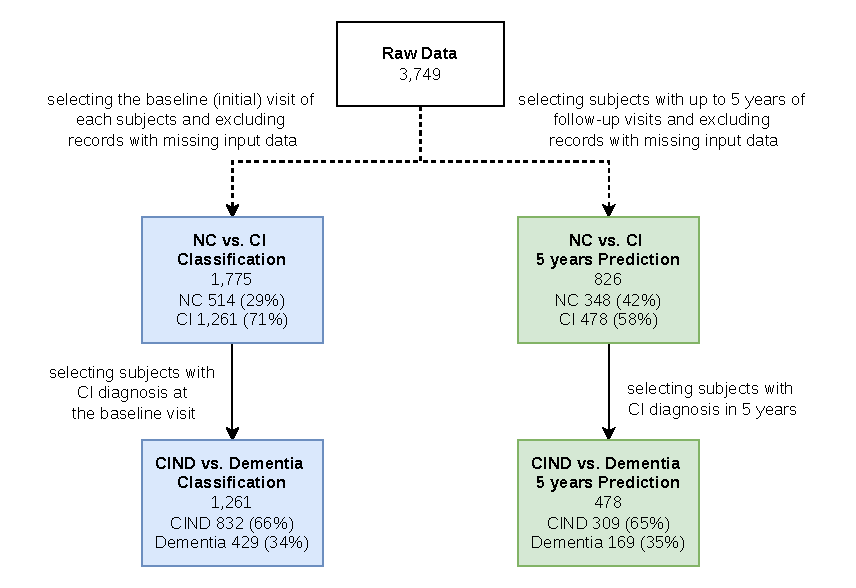
\includegraphics[width=0.7\textwidth]{figures/appendix/class-distribution-adni.pdf}
    \caption{The size of the data and the class distribution in the Alzheimer's Disease Neuroimaging Initiative (ADNI) external datasets}
    \label{fig:adni-data-stat}
\end{figure}

\begin{figure}[ht]
    \centering
    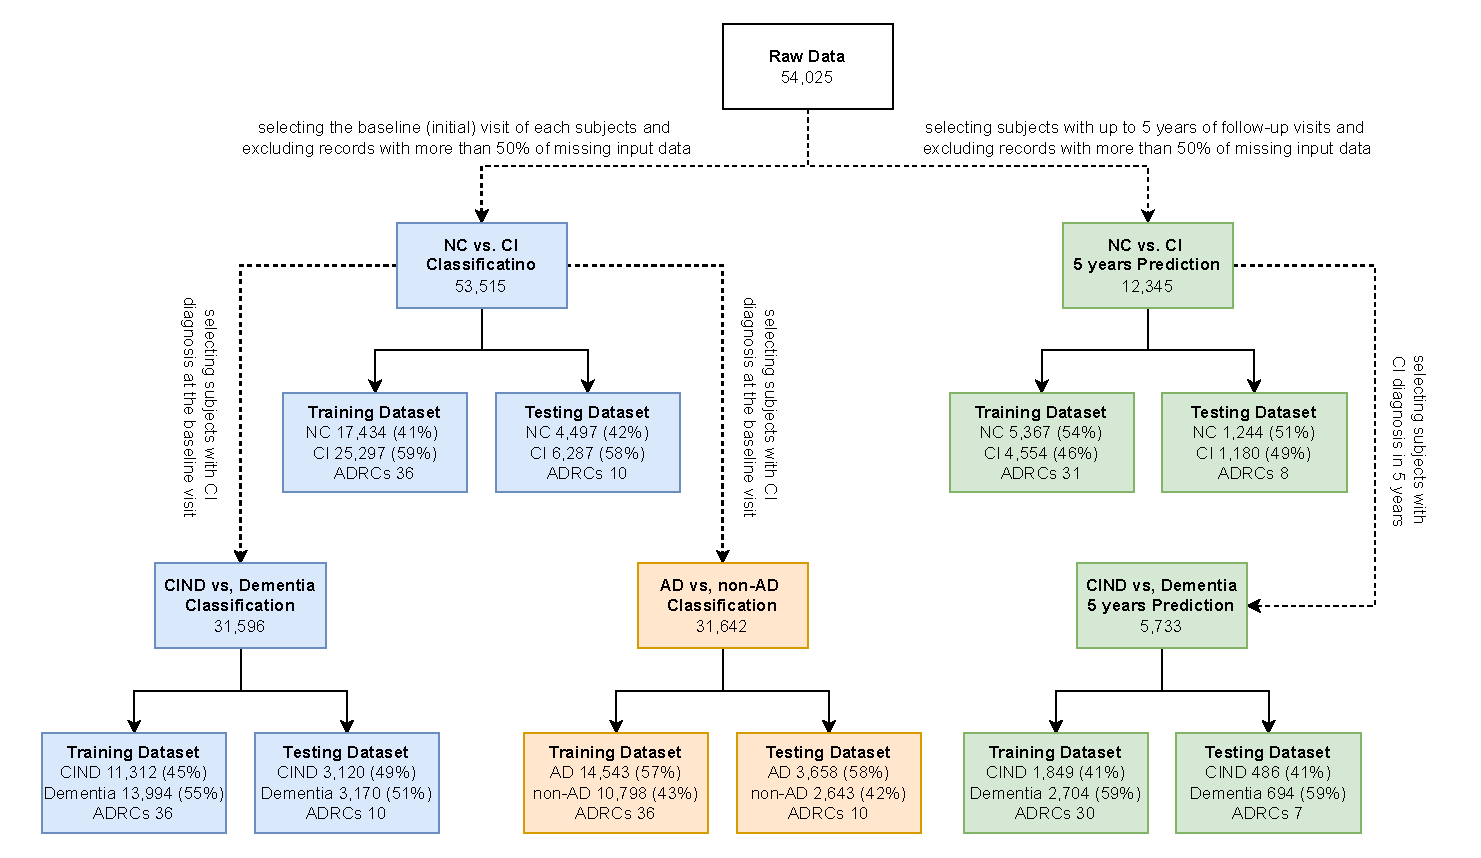
\includegraphics[width=1.0\textwidth]{figures/appendix/class-distribution-nacc.pdf}
    \caption{The size of the data and the class distribution in the NACC training and testing datasets}
    \begin{minipage}{\textwidth}
      \footnotesize The diagram demonstrate the hierarchical selection of data and the data selection criteria in different classification and prediction tasks.\newline
      The training and testing datasets split was done based on Alzheimer's disease research centers (\acrshort{ADRCs}) with 20\% ratio. The training dataset was collected from ADRCs that were not involved in the collection of the holdout testing dataset. The training and testing ADCRs in the NC vs. CI tasks are the same in the following CIND vs. Dementia and AD vs. non-AD tasks.\newline
      The high prevalence of cognitive impairment (\acrshort{CI}) is because subjects participated in NACC study are actively looking for medical advice due to concern on Cognitive deterioration.
    \end{minipage}
    \label{fig:nacc-data-stat}
\end{figure}

\subsection{Feature Selection}\label{sec:feature-selection-apdx}
These features were excluded because they are not available in the Alzheimer's Disease Neuroimaging Initiative (\acrshort{ADNI}) dataset: NACCLIVS, INDEPEND, ABUSOTHR, HEARING, COMPORT, CDRLANG, DECSUB, and DECIN. Categorical features with a dominant category  accounting for 97\% of the samples are excluded. Table~\ref{table:excluded-dominant-features} lists the excluded categories for each classification task. The remaining features were applied to the feature selection method. Table~\ref{table:feature-details} provides details about the selected features in all classification tasks. The correlation of the selected features for each classification task is presented in Figure~\ref{figure:feature-correlation}.

\begin{table}[H]
    \centering
    \caption{List of the excluded features with a dominant category for each classification task}
    \newcolumntype{C}{>{\centering\arraybackslash}X}
    \begin{tabularx}{\textwidth}{|C|C|}
    \hline
        Task & Excluded Features \\ \hline
        NC vs. CI Classificationn & CVCHF, SEIZURES, PD, PDOTHR, NCOTHR \\ \hline
        CIND vs. Dementia Classificationn & CVCHF, PD \\ \hline
        NC vs. CI Prediction & CVCHF, SEIZURES, PD, PDOTHR, DEL, DELSEV, HALL, HALLSEV, ELAT, ELATSEV \\ \hline
        CIND vs. Dementia Prediction & CVCHF, SEIZURES, PD, PDOTHR, HALL, HALLSEV \\ \hline
        AD vs. non-AD Classification & CVCHF, PD \\ \hline
    \end{tabularx}
    \label{table:excluded-dominant-features}
\end{table}


\begin{longtable}{|M{2.5cm}|M{2.5cm}|M{2.5cm}|M{2.5cm}|M{3cm}|}

    \caption{Details of the selected features in all classification tasks}

    \\ \hline
    \textbf{Category} & \textbf{NACC Code} & \textbf{ADNI Code} & \textbf{Description} & \textbf{Categorical \newline Values\textsuperscript{1}}
    \\ \hline
    \endhead
 
    \hline
    \endfoot

    \hline
    \endlastfoot

     % --- Footnotes Section (appears only on the last page) ---
    \hline
    \multicolumn{5}{p{15cm}}{
        \footnotesize This table lists all the selected features across all classification tasks.\newline
        \textsuperscript{1}Continuous features such as age and body mass index (\acrshort{BMI}) do not have categorical values.
    }
    \endlastfoot
    \label{table:feature-details}

    % --- Demographics (3 rows) ---
    \multirow{7}{*}{\parbox{2.5cm}{Demographics}}
     & NACCAGE & entry\_age & Age & ~ \\ \cline{2-5}
     & SEX & PTGENDER & Sex & 0=Male, \newline 1=Female \\ \cline{2-5}
     & PRIMLANG & PTPLANG & Subject's primary language & 0=English, 1=Spanish, 2=Others \\ \hline

    % --- Physical Assessment (1 row) ---
    \multirow{1}{*}{\parbox{2cm}{Physical Assessment}} 
     & NACCBMI & calculated using VSHEIGHT and VSWEIGHT & Body Mass Index (\acrshort{BMI}) & ~ \\ \hline

    \clearpage
    
     % --- Neuropsychiatric Inventory Questionnaire (NPI-Q) (3 rows) ---
    \multirow{3}{*}{\parbox{2cm}{Neuro-psychiatric Inventory Questionnaire (\acrshort{NPI-Q})}} 
     & ANX & NPIE & Anxiety in the last month & \multirow{9}{*}{\parbox{3cm}{0=No, 1=Yes}} \\ \cline{2-4}
     & APP & NPIL & Appetite and eating changes in the last month & \\ \cline{2-4}
     & IRR & NPII & Irritability or lability in the last month & \\ \hline

    % --- Geriatric Depression Scale (GDS) (2 rows) ---
    \multirow{2}{*}{\parbox{2cm}{Geriatric Depression Scale (GDS)}} 
     & MEMPROB & GDMEMORY & Subject reported memory problem & 0=No, 1=Yes \\ \cline{2-5}
     & ENERGY & GDENERGY & Do you feel full of energy? & 0=Yes, 1=No \\ \hline

    % --- Functional Activities Questionnaire (FAQ) (9 rows) ---
    \multirow{9}{*}{\parbox{2cm}{Functional Activities Questionnaire (\acrshort{FAQ}) \newline Instrumental Activities of Daily Living (IADL)}} 
     & BILLS & FAQFINAN & Pay bills and track spending & \multirow{9}{*}{\parbox{3cm}{0=Normal, \newline 1=Never did, \newline 2=Has difficulty but does by self, \newline 3=Requires assistance, \newline 4=Dependent}} \\ \cline{2-4}
     & TAXES & FAQFORM & Assemble tax records & \\ \cline{2-4}
     & SHOPPING & FAQSHOP & Shop alone for necessities & \\ \cline{2-4}
     & GAMES & FAQGAME & Play a game of skill & \\ \cline{2-4}
     & EVENTS & FAQEVENT & Keep track of current events & \\ \cline{2-4}
     & PAYATTN & FAQTV & Pay attention to a conversation & \\ \cline{2-4}
     & REMDATES & FAQREM & Remember dates and appointments & \\ \cline{2-4}
     & TRAVEL & FAQTRAVL & Travel out of neighborhood & \\ \cline{2-4}
     & MEALPREP & FAQMEAL & Prepare a balanced meal & \\ \hline

    % --- Clinical Dementia Rating (CDR) (6 rows) ---
    \multirow{10}{*}{\parbox{2cm}{Clinical Dementia Rating (CDR)}} 
     & MEMORY & CDMEMORY & Memory &  \multirow{10}{*}{\parbox{3cm}{0=No impairment, 1=Questionable impairment, 2=Mild impairment, 3=Moderate impairment, 4=Severe impairment}} \\ \cline{2-4}
     & ORIENT & CDORIENT & Orientation & \\ \cline{2-4}
     & JUDGMENT & CDJUDGE & Judgment \& Problem Solving & \\ \cline{2-4}
     & COMMUN & CDCOMMUN & Community Affairs & \\ \cline{2-4}
     & HOMEHOBB & CDHOME & Home \& Hobbies & \\ \cline{2-4}
     & PERSCARE & CDCARE & Personal Care & \\ \hline

\end{longtable}

% First page - subfigures (a) and (b)
\begin{figure}[H]
    \centering
    \begin{minipage}{0.9\textwidth}
        \centering
        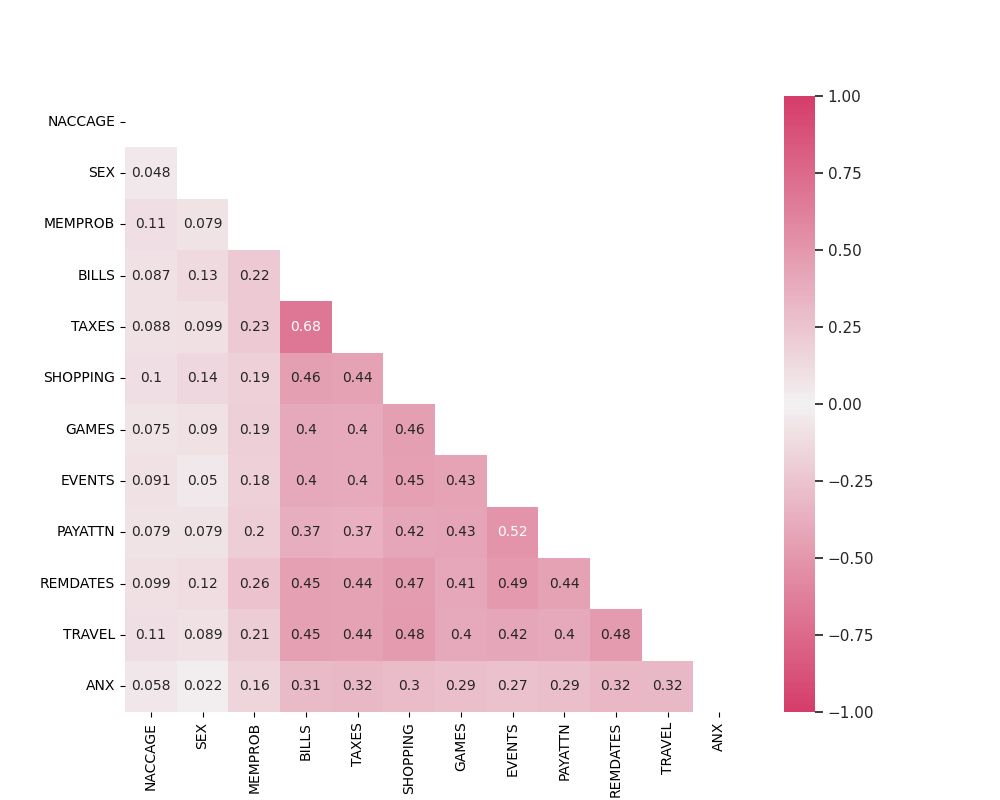
\includegraphics[width=\textwidth]{figures/appendix/impaired_classification_nacc_correlation_matrix.png}
        \caption*{(a) Feature correlation for the NC vs. CI classification task}
        \label{figure:feature-correlation-task1-apdx}
    \end{minipage}
    
    \vspace{0.5cm}
    
    \begin{minipage}{0.9\textwidth}
        \centering
        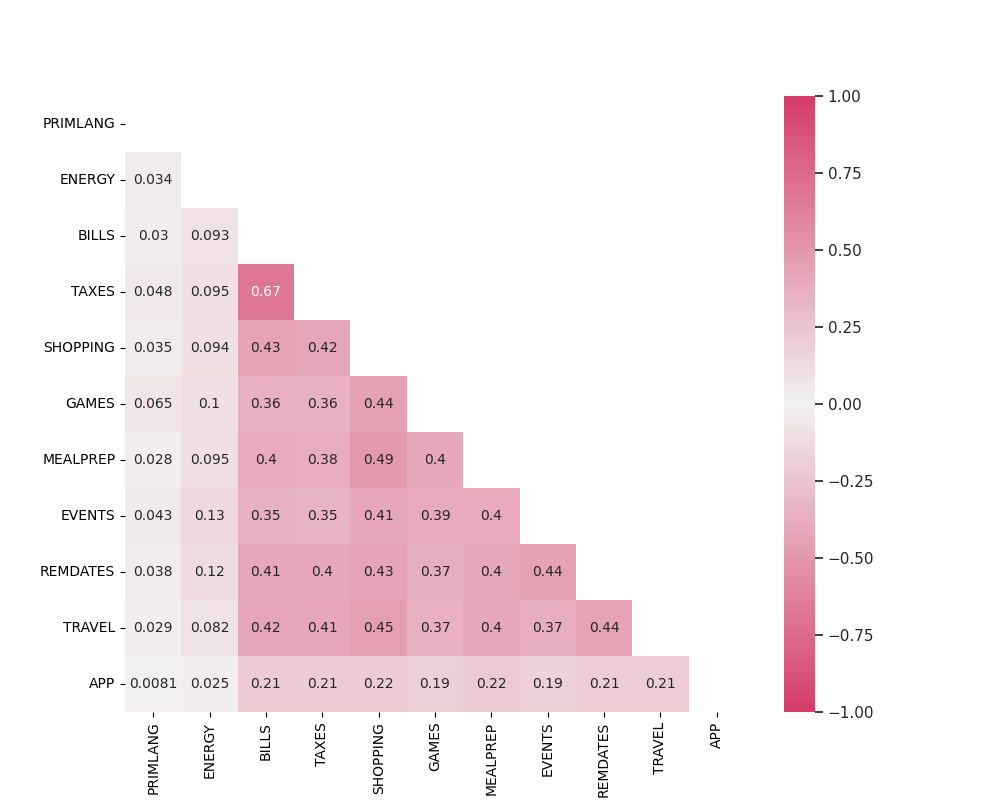
\includegraphics[width=\textwidth]{figures/appendix/dementia_classification_nacc_correlation_matrix.png}
        \caption*{(b) Feature correlation for the CIND vs. dementia classification task}
        \label{figure:feature-correlation-task2-apdx}
    \end{minipage}
    \caption{Feature correlation matrices for different classification and prediction tasks}
    \label{figure:feature-correlation}
\end{figure}

% Second page - subfigures (c) and (d)
\begin{figure}[H]
    \ContinuedFloat
    \centering
    \begin{minipage}{0.9\textwidth}
        \centering
        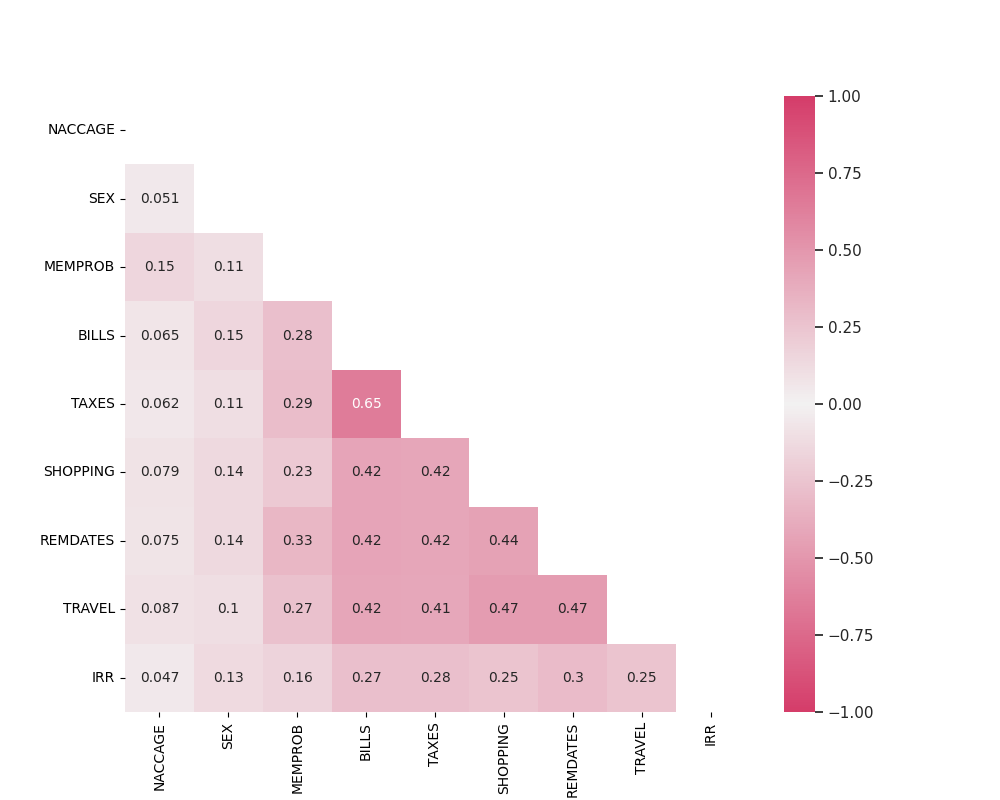
\includegraphics[width=\textwidth]{figures/appendix/impaired_prediction_nacc_correlation_matrix.png}
        \caption*{(c) Feature correlation for the future NC vs. CI prediction task}
        \label{figure:feature-correlation-task3-apdx}
    \end{minipage}
    
    \vspace{0.5cm}
    
    \begin{minipage}{0.9\textwidth}
        \centering
        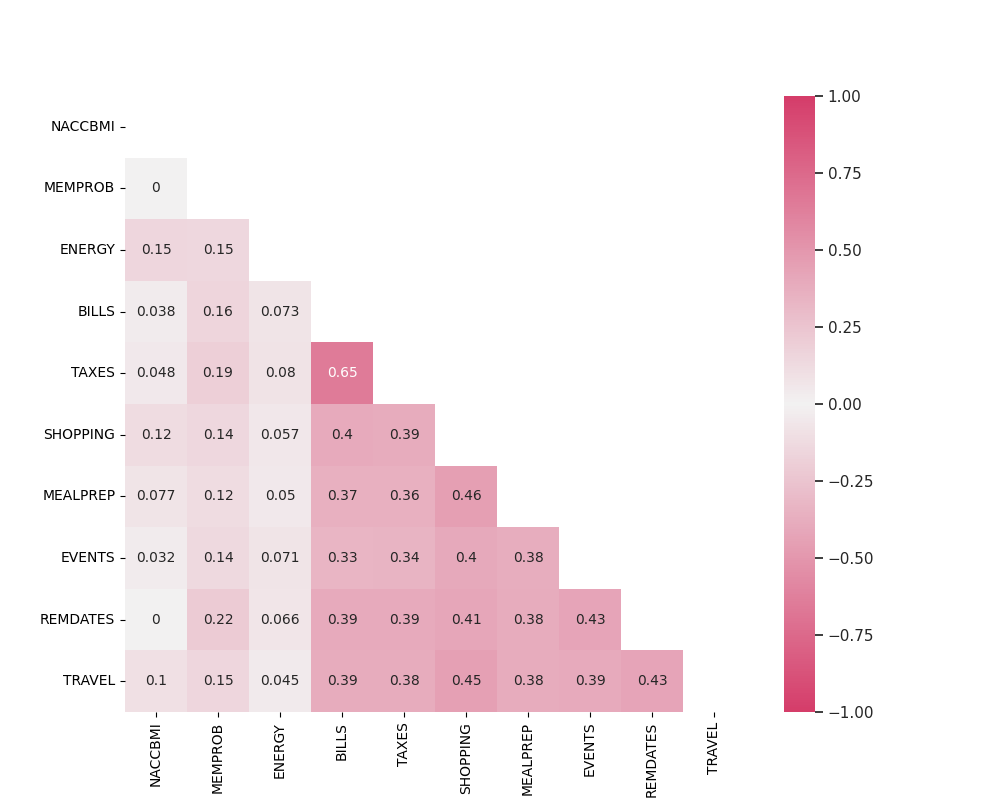
\includegraphics[width=\textwidth]{figures/appendix/dementia_prediction_nacc_correlation_matrix.png}
        \caption*{(d) Feature correlation for the future CIND vs. dementia prediction task}
        \label{figure:feature-correlation-task4-apdx}
    \end{minipage}
    \caption*{Figure \ref{figure:feature-correlation}: Feature correlation matrices for different classification and prediction tasks, continued}
\end{figure}

% Third page - subfigure (e)
\begin{figure}[H]
    \ContinuedFloat
    \centering
    \begin{minipage}{0.9\textwidth}
        \centering
        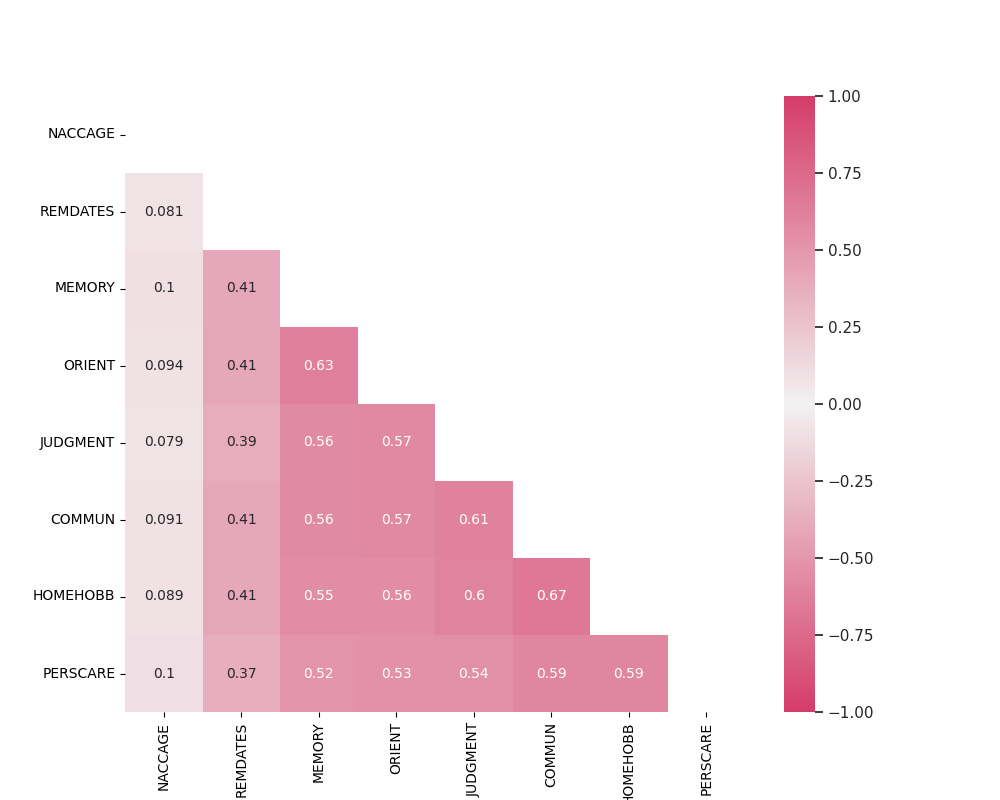
\includegraphics[width=\textwidth]{figures/appendix/type_classification_nacc_correlation_matrix.png}
        \caption*{(e) Feature correlation for the AD vs. non-AD classification task}
        \label{figure:feature-correlation-task5-apdx}
    \end{minipage}
    \caption*{Figure \ref{figure:feature-correlation}: Feature correlation matrices for different classification and prediction tasks (concluded)}
\end{figure}

\section{Supplementary Results of the Logisitic Regression Model Fine-tuning}\label{sec:lr-fine-tuning-apdx}
This section provides supplementary results of the hyperparameters fine-tuning of the selected logisitc regression (\acrshort{LR}) models. The optimization process only fine-tuned the \textit{C} parameter (inverse of the regularization strength). This hyperparameter controls the strength of regularization, which adjusts the balance between model simplicity and prediction accuracy. The \textit{lbfgs} solver was selected as the fixed optimization method due to its computational efficiency and stability for the given dataset size. In addition, the \textit{L2} penalty was exclusively employed. Since a rigorous feature selection phase was already completed prior to this stage, the automatic feature removal capability of the \textit{L1} penalty was not required. Instead, the \textit{L2} penalty was considered sufficient to prevent the model from overfitting and memorizing noise. The following tables (Tables \ref{table:lr-fine-tune-task1-apdx} to \ref{table:lr-fine-tune-task5-apdx}) present the performance and throughput of fine-tuned LR models in all classification tasks. The results demonstrate the ability of the proposed cost-effective model selection algorithm in selecting models that offer the highest efficiency while maintaining a high level of performance.


\begin{table}[H]
    \centering
    \caption{The hyperparameter fine-tuning of the logistic regression model for the NC vs. CI classification task}
    \begin{tabular}{|c|c|c|c|c|M{2cm}|M{2cm}|}
    \hline
        C & F1-score & G-mean & Sensitivity & Specificity & Training Throughput & Prediction Throughput \\ \hline
        5 & 0.848 & 0.842 & 0.785 & 0.903 & 1,511,839 \newline (1.07x) & 24,641,680\newline(1.09x) \\ \hline
        0.1 & 0.847 & 0.842 & 0.782 & 0.906 & 1,525,704\newline(1.08x) & 24,251,600\newline(1.07x) \\ \hline
        1 & 0.848 & 0.842 & 0.785 & 0.904 & 1,418,872 & 22,620,340 \\ \hline
        10 & 0.848 & 0.842 & 0.785 & 0.903 & 1,372,488\newline(0.97x) & 22,183,611\newline(0.98x) \\ \hline
        0.01c & 0.843 & 0.840 & 0.769 & 0.918 & 1,551,843\newline(1.09x) & 20,912,796\newline(0.92x) \\ \hline
    \multicolumn{7}{p{400pt}}{\footnotesize The \textit{C} parameter is the only fine-tuned hyperparameter. Default values are used for the other hyperparameters as defined in sklearn Python library. The most cost-effective model is when \textit{C} set as 5. This resulted in 1.07 increase in training throughput and 1.09 increase in prediction throughput as compared to the best performing model of \textit{C} equals 1 with similar level of performance.}
    \end{tabular}
    \label{table:lr-fine-tune-task1-apdx}
\end{table}

\begin{table}[H]
    \centering
    \caption{The hyperparameter fine-tuning of the logistic regression model for the CIND vs. dementia classification task}
    \begin{tabular}{|c|c|c|c|c|M{2cm}|M{2cm}|}
    \hline
        C & F1-score & G-mean & Sensitivity & Specificity & Training Throughput & Prediction Throughput \\ \hline
        0.01 & 0.842 & 0.828 & 0.827 & 0.830 & 512,085 & 19,831,465 \\ \hline
        0.1 & 0.842 & 0.828 & 0.827 & 0.829 & 434,190 (0.85x) & 17,929,038 (0.90x) \\ \hline
        1 & 0.842 & 0.828 & 0.827 & 0.829 & 565,870 (1.11x) & 17,314,929 (0.87x) \\ \hline
        5 & 0.842 & 0.828 & 0.827 & 0.829 & 579,724 (1.13x) & 17,300,820 (0.87x) \\ \hline
        10 & 0.842 & 0.828 & 0.827 & 0.829 & 586,756 (1.15x) & 17,351,721 (0.87x) \\ \hline
    \multicolumn{7}{p{400pt}}{\footnotesize The \textit{C} parameter is the only fine-tuned hyperparameter. Default values are used for the other hyperparameters as defined in sklearn Python library. The most cost-effective model is when \textit{C} set as 0.01.}
    \end{tabular}
    \label{table:lr-fine-tune-task2-apdx}
\end{table}

\begin{table}[H]
    \centering
    \caption{The hyperparameter fine-tuning of the logistic regression model for the future NC vs. CI prediction task}
    \begin{tabular}{|c|c|c|c|c|M{2cm}|M{2cm}|}
    \hline
        C & F1-score & G-mean & Sensitivity & Specificity & Training Throughput & Prediction Throughput \\ \hline
        5 & 0.747 & 0.770 & 0.723 & 0.820 & 819,113 (1.04x) & 6,630,848 (1.07x) \\ \hline
        0.1 & 0.747 & 0.771 & 0.718 & 0.828 & 784,029 & 6,173,582 \\ \hline
        1 & 0.747 & 0.770 & 0.723 & 0.821 & 755,493 (0.96x) & 6,543,298 (0.99x) \\ \hline
        10 & 0.747 & 0.770 & 0.723 & 0.820 & 783,967 (0.99x) & 7,094,149 (1.07x) \\ \hline
        0.01 & 0.744 & 0.770 & 0.692 & 0.858 & 885,304 (1.13x) & 5,473,828 (0.83x) \\ \hline
    \multicolumn{7}{p{400pt}}{\footnotesize The \textit{C} parameter is the only fine-tuned hyperparameter. Default values are used for the other hyperparameters as defined in sklearn Python library. The most cost-effective model is when \textit{C} set as 5. This resulted in 1.04 increase in training throughput and 1.07 increase in prediction throughput as compared to the best performing model of \textit{C} equals 0.1 with similar level of performance.}
    \end{tabular}
    \label{table:lr-fine-tune-task3-apdx}
\end{table}

\begin{table}[H]
    \centering
    \caption{The hyperparameter fine-tuning of the logistic regression model for the future CIND vs. dementia prediction task}
    \begin{tabular}{|c|c|c|c|c|M{2cm}|M{2cm}|}
    \hline
        C & F1-score & G-mean & Sensitivity & Specificity & Training Throughput & Prediction Throughput \\ \hline
        0.01 & 0.773 & 0.757 & 0.714 & 0.804 & 744,495 (1.14x) & 5,276,181 (1.41x) \\ \hline
        10 & 0.785 & 0.763 & 0.738 & 0.788 & 757,565 (1.16x) & 4,915,115 (1.32x) \\ \hline
        5 & 0.785 & 0.763 & 0.738 & 0.788 & 705,062 (1.08x) & 4,750,137 (1.27x) \\ \hline
        1 & 0.785 & 0.763 & 0.739 & 0.788 & 655,482 & 3,732,914 \\ \hline
        0.1 & 0.782 & 0.760 & 0.736 & 0.786 & 636,293 (0.97x) & 4,396,008 (1.18x) \\ \hline
    \multicolumn{7}{p{400pt}}{\footnotesize The \textit{C} parameter is the only fine-tuned hyperparameter. Default values are used for the other hyperparameters as defined in sklearn Python library. The most cost-effective model is when \textit{C} set as 0.01. This resulted in 1.14 increase in training throughput and 1.41 increase in prediction throughput as compared to the best performing model of \textit{C} equals 1 with similar level of performance.}
    \end{tabular}
    \label{table:lr-fine-tune-task4-apdx}
\end{table}

\begin{table}[H]
    \centering
    \caption{The hyperparameter fine-tuning of the logistic regression model for the AD vs. non-AD classification task}
    \begin{tabular}{|c|c|c|c|M{2cm}|M{2cm}|}
    \hline
        C & G-mean & Sensitivity & Specificity & Training Throughput & Prediction Throughput \\ \hline
        5 & 0.702 & 0.689 & 0.714 & 1,123,435 (1.34x) & 19,910,963 (1.20x) \\ \hline
        10 & 0.702 & 0.689 & 0.714 & 1,127,797 (1.35x) & 19,810,778 (1.20x) \\ \hline
        0.1 & 0.701 & 0.688 & 0.715 & 1,105,503 (1.32x) & 18,360,040 (1.11x) \\ \hline
        1 & 0.702 & 0.689 & 0.715 & 1,124,573 (1.34x) & 17,661,511 (1.07x) \\ \hline
        0.01 & 0.702 & 0.686 & 0.718 & 837,734 & 16,524,892 \\ \hline
    \multicolumn{6}{p{350pt}}{\footnotesize The \textit{C} parameter is the only fine-tuned hyperparameter. Default values are used for the other hyperparameters as defined in sklearn Python library. The most cost-effective model is when \textit{C} set as 5. This resulted in 1.34 increase in training throughput and 1.20 increase in prediction throughput as compared to the best performing model of \textit{C} equals 0.01 with similar level of performance.}
    \end{tabular}
    \label{table:lr-fine-tune-task5-apdx}
\end{table}

\section{Cost-effective Model Selection Algorithm Use Cases}\label{sec:selection-algorithm-usecases-apdx}
In order to demonstrate how the proposed model selection algorithm can help identify the most cost-effective model that aligns with specific use case requirements, Table~\ref{table:selection-algorithm-usecases} provides a comparison of performance and speed requirements across various use cases from different industries. It is important to note that the metrics and requirements presented in this table are mainly for illustrative purposes and should not be used as a definitive guide.

\begin{table}[!ht]
    \centering
    \caption{Comparison of performance and speed requirements across diverse use cases}
    \newcolumntype{C}{>{\centering\arraybackslash}X}
    \begin{tabularx}{\textwidth}{|C|C|C|C|C|}
    \hline
        \textbf{Use Case} & \textbf{Performance Metrics} & \textbf{Primary Metric} &  \textbf{Speed Requirement} & \textbf{Cost-effectiveness Requirement} \\ \hline
        Healthcare --- Disease Prediction & F2-score and Accuracy & F2-score & Prediction speed is more important than training speed & Minor decrease in performance for any degree of improvement in speed \\ \hline
        Finance --- Credit Scoring & F1-score and AUC & F1-score & Both training and prediction speed are equally important & Minor decrease in performance for high improvement in speed \\ \hline
        Retail --- Customer Churn Prediction & F1-score and Recall & F1-score & Prediction speed is more important than training speed & Minor decrease in performance for any degree of improvement in speed \\ \hline
        Manufacturing --- Fault Detection & F2-score & F2-score & Prediction speed is more important than training speed & Moderate decrease in performance for high improvement in speed \\ \hline
        Telecomm-unications --- Network Anomaly Detection & F2-score and AUC & F2-score & Both training and prediction speed are equally important & Moderate decrease in performance for high improvement in speed \\ \hline
    \end{tabularx}
    \label{table:selection-algorithm-usecases}
\end{table}

Each business use case has unique performance requirements that need to be taken into account when developing machine learning models. For the prediction of diseases in healthcare care, a high F2-score is essential to ensure that the models correctly identify positive cases. Therefore, the F2-score should be considered as the primary metric to assess such models. In retail, customer churn prediction models with high F1-score are crucial, especially in uneven class distributions. Recall can be used as a secondary metric to measure the model's ability to identify customers at risk of churn. On the other hand, the F2-score is considered the most critical performance metric to evaluate the ability of network anomaly detection models to identify as many anomalies as possible. The AUC is a valuable additional measure to distinguish between normal and anomalous activities. The machine learning model fine-tuning process can be complicated when multiple performance metrics are used to evaluate the models. Model developers can utilize the proposed model selection algorithm to simplify the process. The algorithm selects the best-performing model based on the defined performance metrics and their appropriate weights according to the unique use case requirements.

Besides performance, The speed of the machine learning models is another crucial evaluation metric for use cases requiring efficient solutions. The speed of the model may have an impact on the cost of training and using the model, especially if the model is developed and deployed in a cloud infrastructure. Different use cases may have different requirements for training and prediction speed. In healthcare, especially in disease prediction applications, the speed of prediction is critical to timely treatment decisions and to reduce the cost of widely serving the model. While training the model may be a time-consuming process, it typically occurs offline and does not directly impact patient care. In contrast, financial institutions often retrain credit scoring models to adapt to changing conditions. Therefore, it is important to have a fast training speed and prediction speed to enable quick responses. In other scenarios where machine learning models are being evaluated and optimized through multiple iterations and tests, such as model experiments in research, the speed of training is more crucial. Optimizing the model hyperparameters with different requirements of model training and prediction speed can be challenging and time-consuming. The proposed model selection algorithm automates the process by selecting models with the highest speed based on defined weights of training and prediction throughputs.

An ideal solution is one that delivers the desired results efficiently and effectively. There is often a delicate balance between model performance and efficiency, as highly performing models typically possess complex architectures that demand significant resources and time for training and inference. It is essential to select models that align with the specific performance and efficiency needs of the business use cases. Certain critical use cases, such as disease prediction, require highly accurate models, while model speed is also important in emergency situations. In these cases, an ideal model balances both factors without significantly sacrificing model performance. On the other hand, a model that is slightly less accurate but significantly faster can be a reliable option for applications that frequently scan large volumes of records, such as credit scoring models. There are other use cases where less accurate, yet admirably fast, models can be used. For instance, fault detection systems in manufacturing aim to quickly identify potential issues to prevent downtime. The speed of detection is crucial, even if it means having higher false positives, as it ensures immediate attention and further inspection. Selecting the appropriate model hyperparameters to achieve the desired level of performance and efficiency can be a challenging task. The proposed model selection algorithm can be useful in this regard. By transforming the model performance and efficiency requirements into preferred thresholds, the algorithm streamlines the selection of cost-effective models that align with the business needs.

\section{Supplementary Performance Results of the Selected Logistic Regression Model}
\label{sec:lr-complete-perf-apdx}
This section provides an extended report of the performance of the LR models. Tables \ref{table:lr-complete-perf-task1-apdx} to \ref{table:lr-complete-perf-task5-apdx} present the performance of the LR models in all classification tasks using additional metrics.

\begin{table}[H]
    \centering
    \caption{Extended performance metrics of the selected logistic regression model for the NC vs. CI classification task}
    \newcolumntype{C}{>{\centering\arraybackslash}X}
    \begin{tabularx}{\textwidth}{|C|C|C|C|}
    \hline
        \textbf{Metric} & \textbf{Internal Cross-Validation} & \textbf{NACC Cross-center Validation} & \textbf{ADNI External Validation} \\ \hline
        F1-score & 0.848 & 0.823 & 0.833 \\ \hline
        G-mean & 0.842 & 0.809 & 0.820 \\ \hline
        Precision & 0.922 & 0.874 & 0.953 \\ \hline
        Sensitivity & 0.785 & 0.777 & 0.739 \\ \hline
        Specificity & 0.903 & 0.843 & 0.911 \\ \hline
        Accuracy & 0.833 & 0.805 & 0.789 \\ \hline
        AUC & 0.844 & 0.810 & 0.825 \\ \hline
        AUPRC & 0.851 & 0.809 & 0.890 \\ \hline
        Kappa & 0.666 & 0.607 & 0.559 \\ \hline
    \multicolumn{4}{p{400pt}}{\footnotesize G-mean: geometric mean score, AUC: area under the curve, AUPRC: area under the precision-recall curve, Kappa: Cohen's kappa score.}
    \end{tabularx}
    \label{table:lr-complete-perf-task1-apdx}
\end{table}

\begin{table}[H]
    \centering
    \caption{Extended performance metrics of the selected logistic regression model for the CIND vs. dementia classification task}
    \newcolumntype{C}{>{\centering\arraybackslash}X}
    \begin{tabularx}{\textwidth}{|C|C|C|C|}
    \hline
        \textbf{Metric} & \textbf{Internal Cross-Validation} & \textbf{NACC Cross-center Validation} & \textbf{ADNI External Validation} \\ \hline
        F1-score & 0.842 & 0.837 & 0.777 \\ \hline
        G-mean & 0.828 & 0.826 & 0.840 \\ \hline
        Precision & 0.857 & 0.802 & 0.690 \\ \hline
        Sensitivity & 0.827 & 0.874 & 0.888 \\ \hline
        Specificity & 0.830 & 0.782 & 0.794 \\ \hline
        Accuracy & 0.828 & 0.828 & 0.826 \\ \hline
        AUC & 0.828 & 0.828 & 0.841 \\ \hline
        AUPRC & 0.804 & 0.765 & 0.651 \\ \hline
        Kappa & 0.654 & 0.656 & 0.638 \\ \hline
    \multicolumn{4}{p{400pt}}{\footnotesize G-mean: geometric mean score, AUC: area under the curve, AUPRC: area under the precision-recall curve, Kappa: Cohen's kappa score.}
    \end{tabularx}
    \label{table:lr-complete-perf-task2-apdx}
\end{table}

\begin{table}[H]
    \centering
    \caption{Extended performance metrics of the selected logistic regression model for the future NC vs. CI prediction task}
    \newcolumntype{C}{>{\centering\arraybackslash}X}
    \begin{tabularx}{\textwidth}{|C|C|C|C|}
    \hline
        \textbf{Metric} & \textbf{Internal Cross-Validation} & \textbf{NACC Cross-center Validation} & \textbf{ADNI External Validation} \\ \hline
        F1-score & 0.747 & 0.772 & 0.791 \\ \hline
        G-mean & 0.770 & 0.787 & 0.777 \\ \hline
        Precision & 0.774 & 0.829 & 0.844 \\ \hline
        Sensitivity & 0.723 & 0.721 & 0.745 \\ \hline
        Specificity & 0.820 & 0.859 & 0.810 \\ \hline
        Accuracy & 0.776 & 0.792 & 0.772 \\ \hline
        AUC & 0.772 & 0.790 & 0.778 \\ \hline
        AUPRC & 0.686 & 0.734 & 0.776 \\ \hline
        Kappa & 0.546 & 0.582 & 0.543 \\ \hline
    \multicolumn{4}{p{400pt}}{\footnotesize G-mean: geometric mean score, AUC: area under the curve, AUPRC: area under the precision-recall curve, Kappa: Cohen's kappa score.}
    \end{tabularx}
    \label{table:lr-complete-perf-task3-apdx}
\end{table}

\begin{table}[H]
    \centering
    \caption{Extended performance metrics of the selected logistic regression model for the future CIND vs. dementia prediction task}
    \newcolumntype{C}{>{\centering\arraybackslash}X}
    \begin{tabularx}{\textwidth}{|C|C|C|C|}
    \hline
        \textbf{Metric} & \textbf{Internal Cross-Validation} & \textbf{NACC Cross-center Validation} & \textbf{ADNI External Validation} \\ \hline
        F1-score & 0.773 & 0.811 & 0.715 \\ \hline
        G-mean & 0.757 & 0.803 & 0.780 \\ \hline
        Precision & 0.842 & 0.887 & 0.655 \\ \hline
        Sensitivity & 0.714 & 0.746 & 0.787 \\ \hline
        Specificity & 0.804 & 0.864 & 0.773 \\ \hline
        Accuracy & 0.750 & 0.795 & 0.778 \\ \hline
        AUC & 0.759 & 0.805 & 0.780 \\ \hline
        AUPRC & 0.771 & 0.811 & 0.591 \\ \hline
        Kappa & 0.500 & 0.591 & 0.536 \\ \hline
    \multicolumn{4}{p{400pt}}{\footnotesize G-mean: geometric mean score, AUC: area under the curve, AUPRC: area under the precision-recall curve, Kappa: Cohen's kappa score.}
    \end{tabularx}
    \label{table:lr-complete-perf-task4-apdx}
\end{table}

\begin{table}[H]
    \centering
    \caption{Extended performance metrics of the selected logistic regression model for the AD vs. non-AD classification task}
    \newcolumntype{C}{>{\centering\arraybackslash}X}
    \begin{tabularx}{\textwidth}{|C|C|C|}
    \hline
        \textbf{Metric} & \textbf{Internal Cross-Validation} & \textbf{NACC Cross-center Validation} \\ \hline
        F1-score & 0.725 & 0.706 \\ \hline
        G-mean & 0.702 & 0.670 \\ \hline
        Precision & 0.765 & 0.735 \\ \hline
        Sensitivity & 0.689 & 0.679 \\ \hline
        Specificity & 0.714 & 0.660 \\ \hline
        Accuracy & 0.700 & 0.671 \\ \hline
        AUC & 0.702 & 0.670 \\ \hline
        AUPRC & 0.705 & 0.686 \\ \hline
        Kappa & 0.397 & 0.334 \\ \hline
    \multicolumn{3}{p{400pt}}{\footnotesize G-mean: geometric mean score, AUC: area under the curve, AUPRC: area under the precision-recall curve, Kappa: Cohen's kappa score.}
    \end{tabularx}
    \label{table:lr-complete-perf-task5-apdx}
\end{table}

\section{Supplementary Results of Model Explainability}\label{sec:xai-apdx}
This section provides supplementary results related to the model explainability phase of this study. It is intended to support the findings that were discussed previously in the results and analysis chapter. The feature importance in the NACC cross-center validation and the ADNI external validation for all classification tasks is presented in Figures \ref{figure:summary-plot-task1-apdx} to \ref{figure:summary-plot-task5-apdx} together with summary plots demonstrating the direction of the impact of the features. Figures \ref{figure:dice-nacc-task1-apdx} to \ref{figure:dice-nacc-task4-apdx} display the quantity (the number of counterfactual examples generated per instance) and the sparsity (the number of features needed to be changed to generate the counterfactual examples) of the counterfactual explanation in the NACC cross-center validation, which can be compared with the corresponding metrics in the ADNI external validation that were provided previously in the results and analysis chapter. Tables \ref{table:cfe-adni-task1-apdx} to \ref{table:cfe-adni-task4-apdx} demonstrate samples of counterfactual examples generated in the ADNI external validation for all classification tasks to illustrate the feature changes required to reverse the predicted outcomes. The Diverse Counterfactual Explanations (\acrshort{DiCE}) with the \acrshort{KD-Tree} (K-dimensional tree) search method was used to generate the counterfactual examples for all classification tasks except the future CIND vs. dementia prediction task which used the random search method.

\begin{figure}[H]
    \centering
    \begin{minipage}{0.48\textwidth}
        \centering
        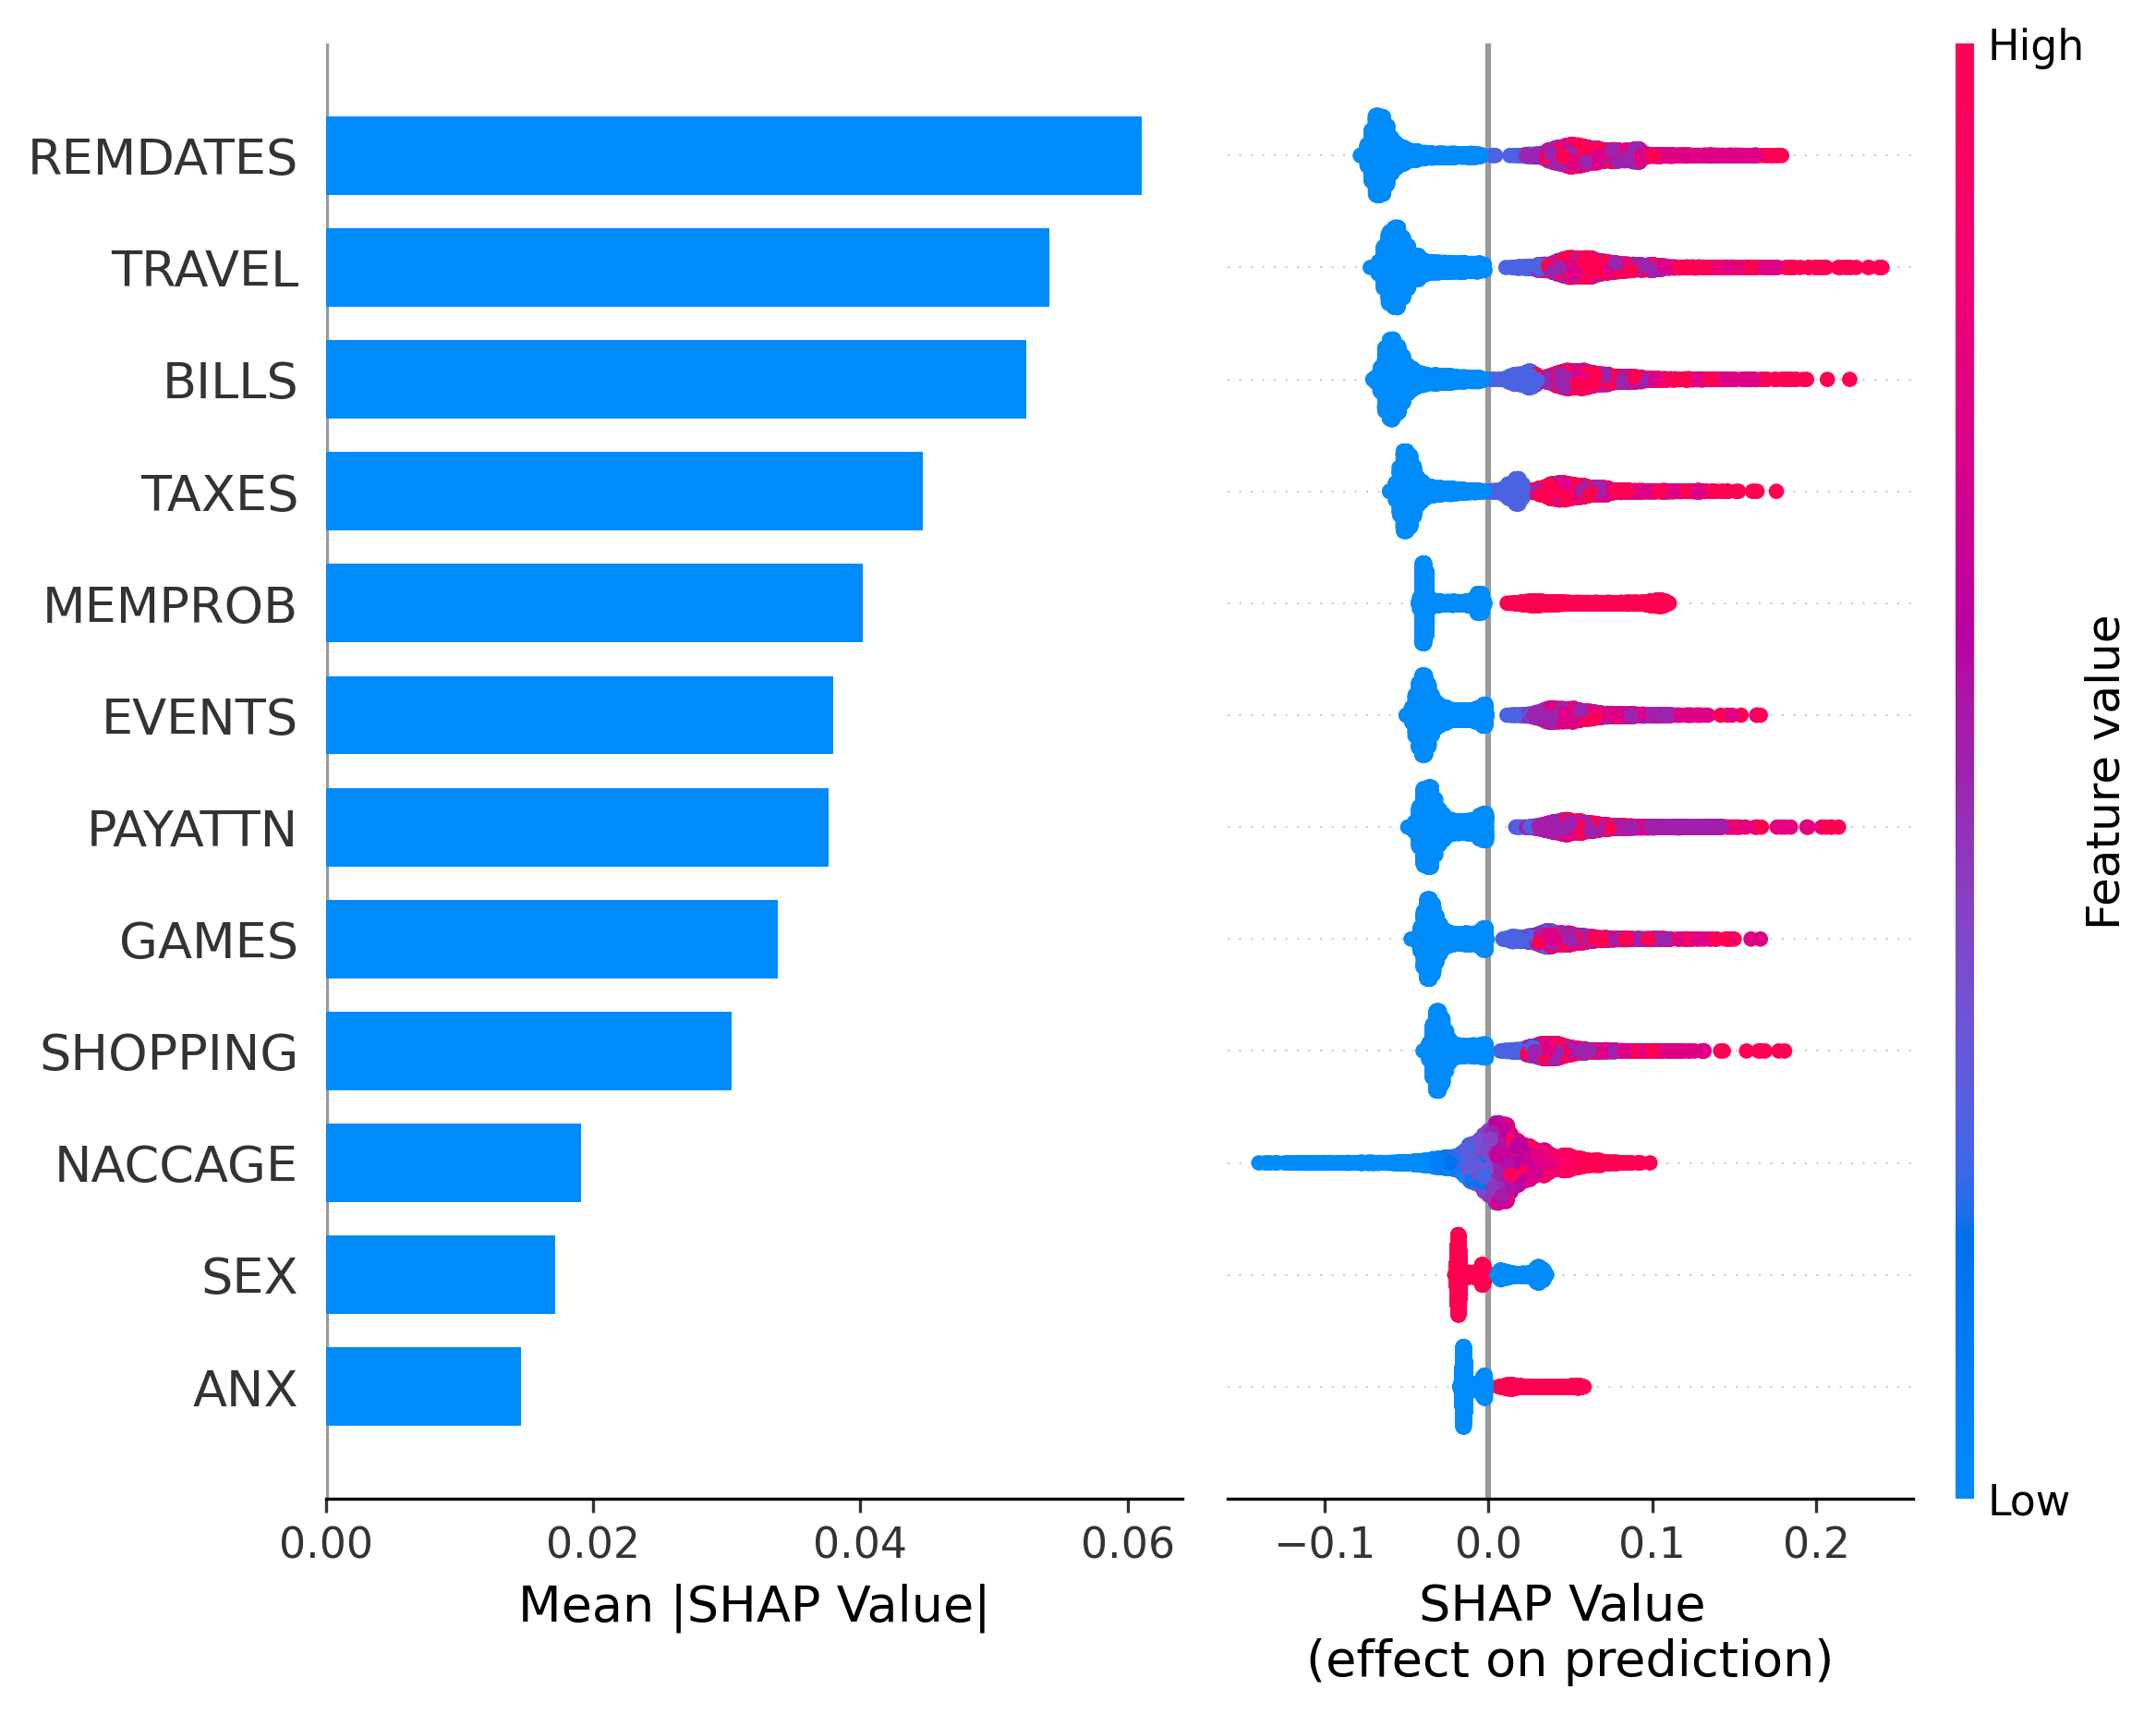
\includegraphics[width=\textwidth]{figures/appendix/impaired_classification_nacc_shap_feature_importance.png}
        \caption*{(a)  NACC cross-center validation}
    \end{minipage}
    \begin{minipage}{0.48\textwidth}
        \centering
        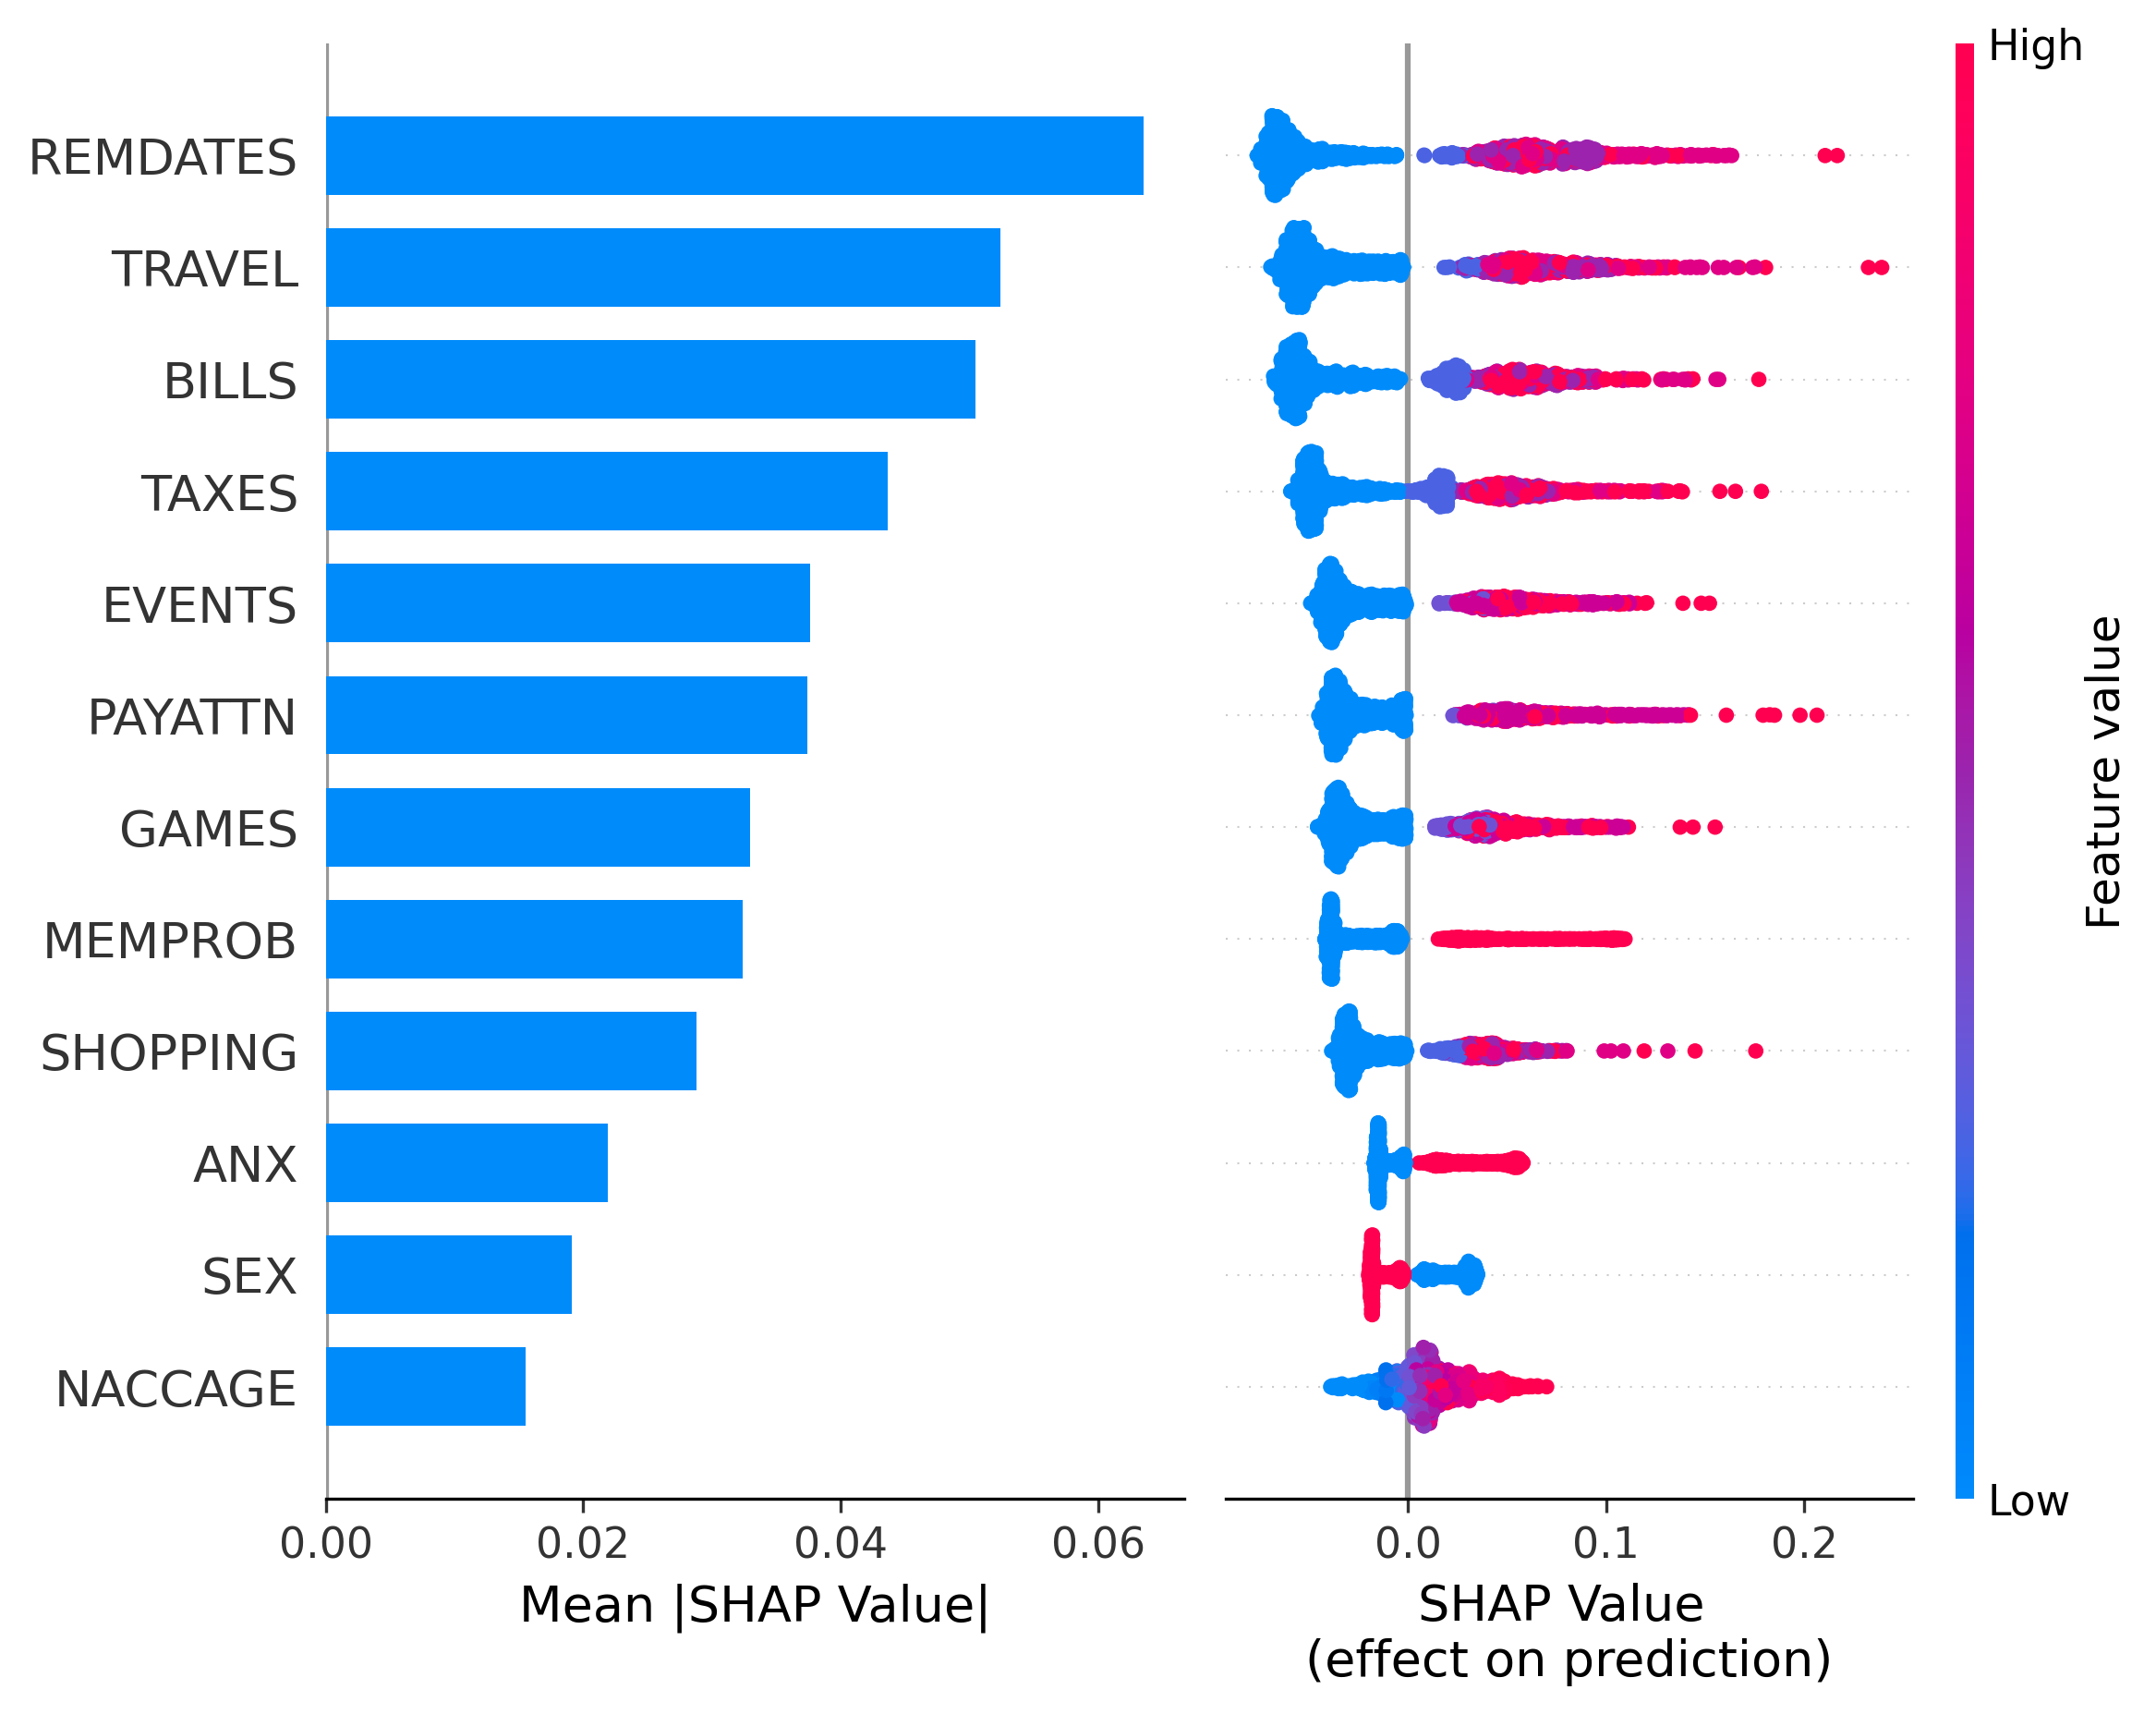
\includegraphics[width=\textwidth]{figures/appendix/impaired_classification_adni_shap_feature_importance.png}
        \caption*{(b) ADNI External Validation}
    \end{minipage}
    \caption{Feature importance with summary plot for the NC vs. CI classification task}
    \label{figure:summary-plot-task1-apdx}
\end{figure}

\begin{figure}[H]
    \centering
    \begin{minipage}{0.48\textwidth}
        \centering
        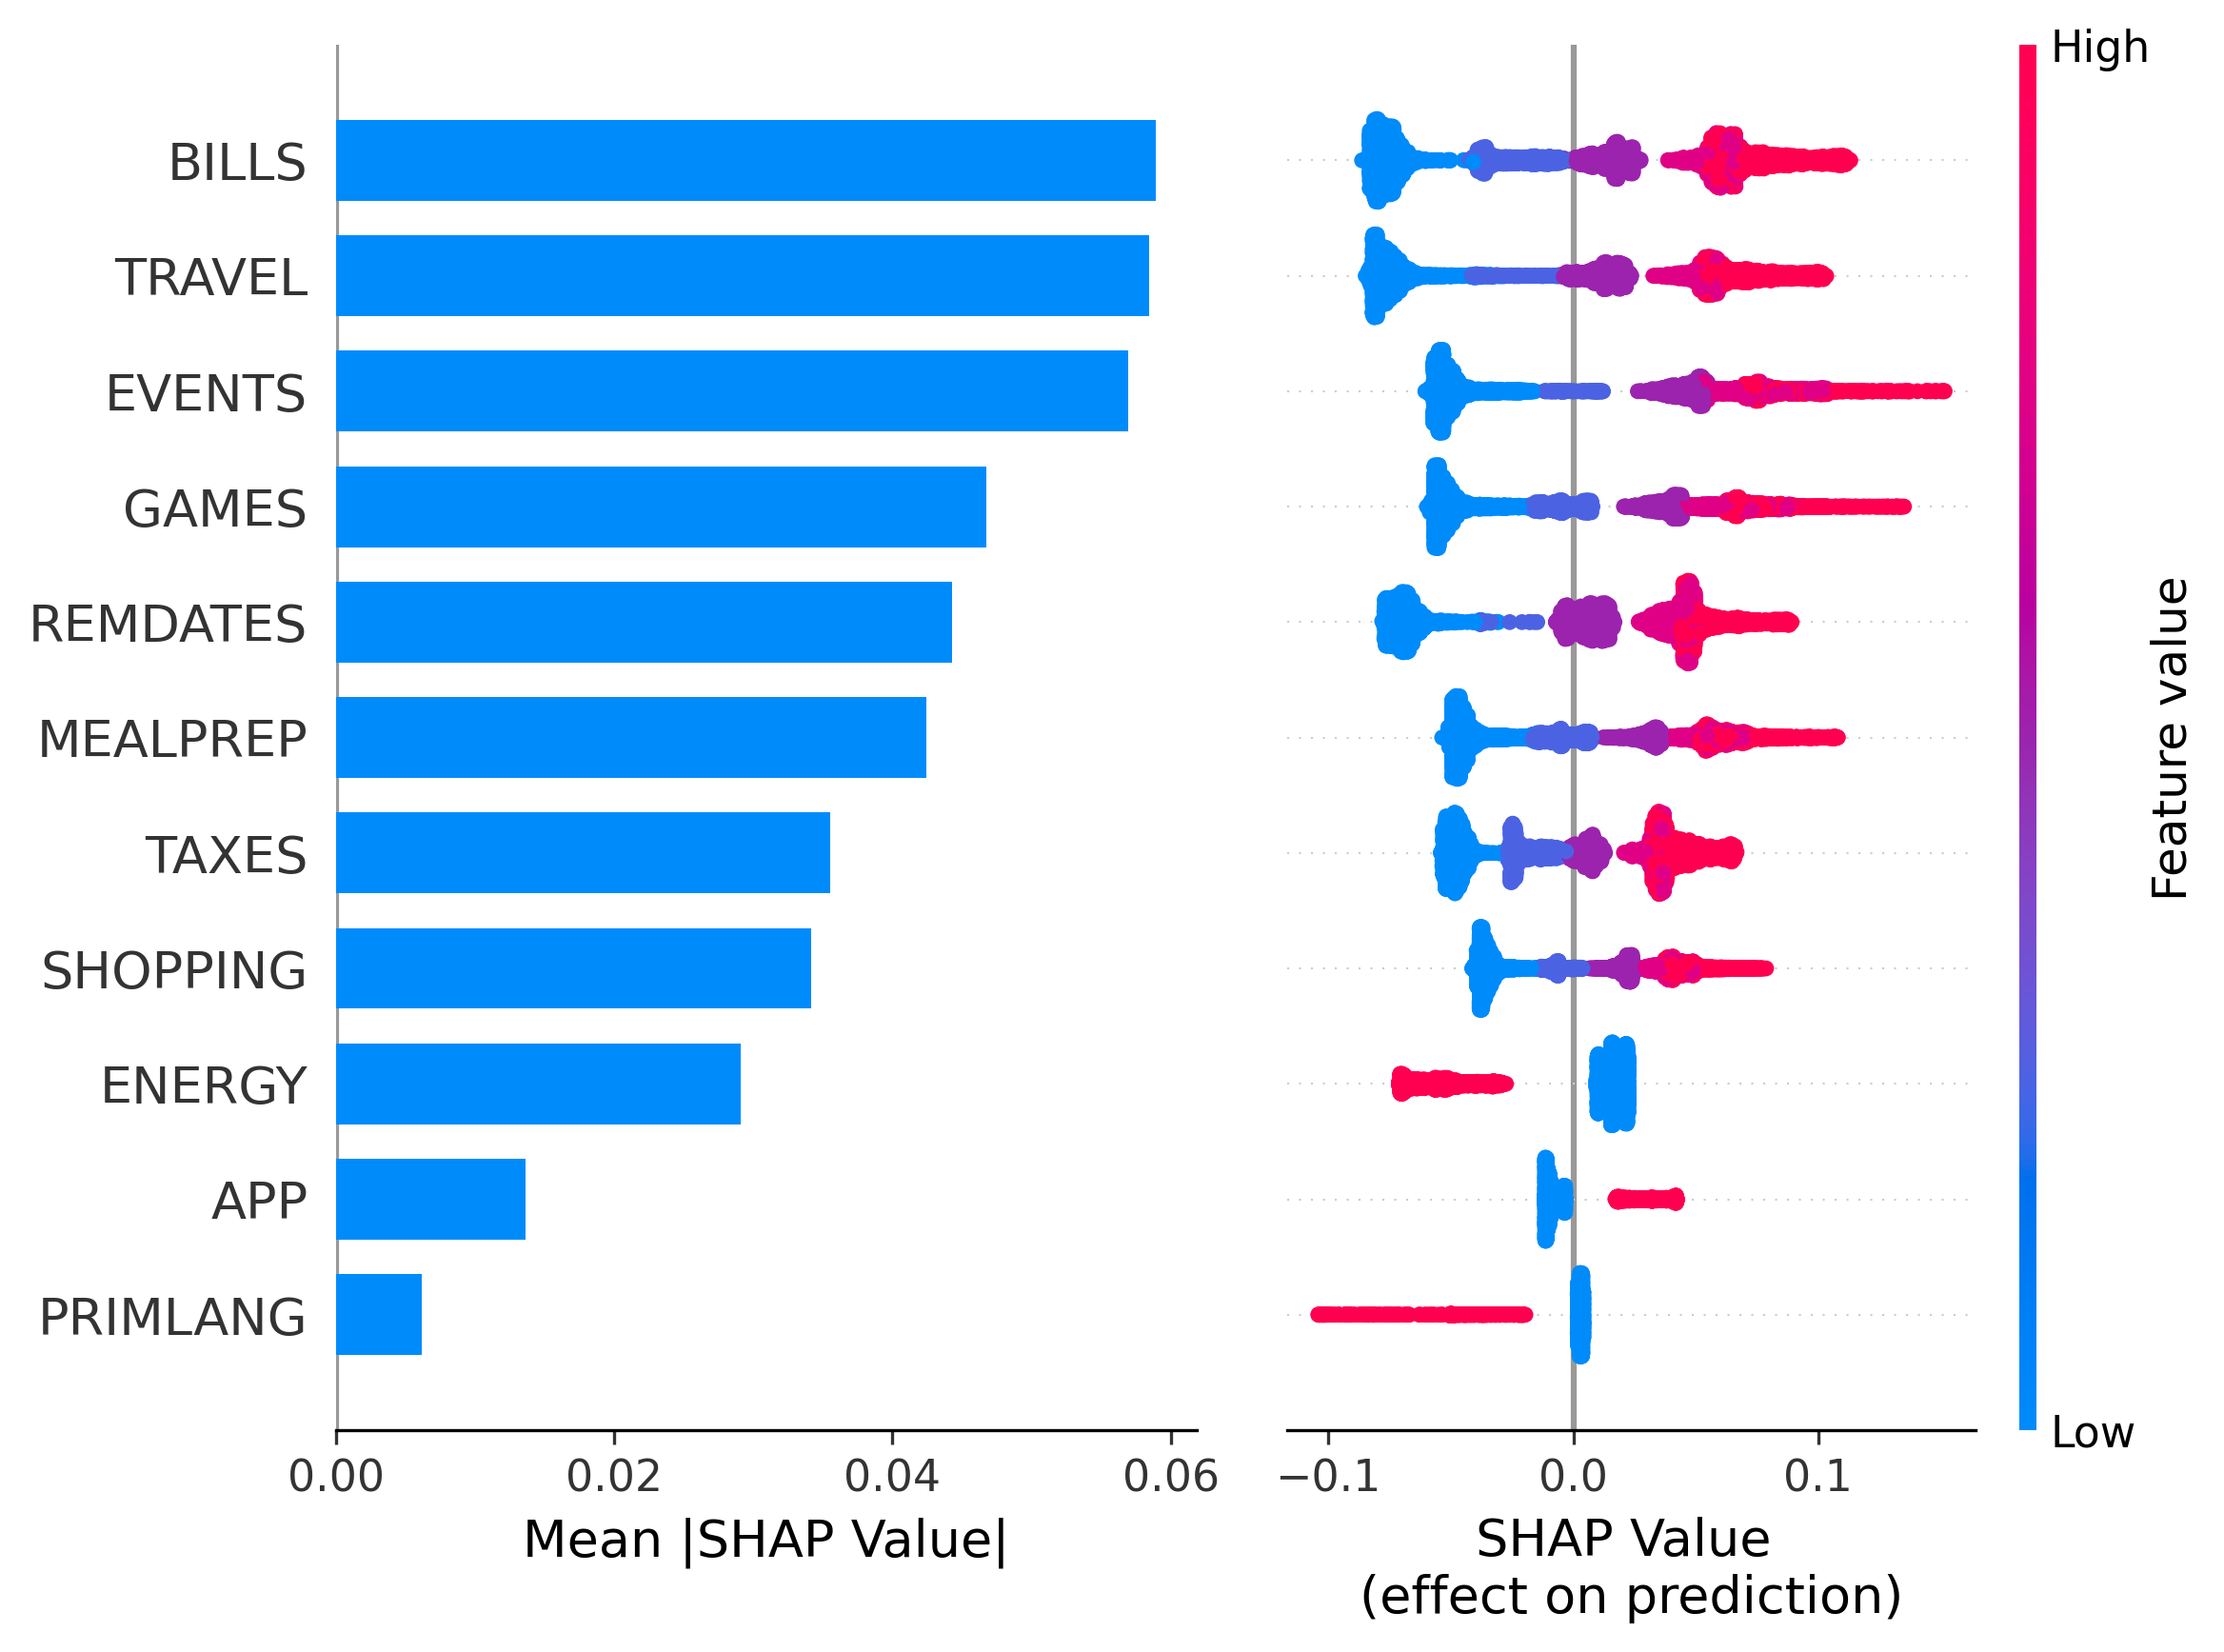
\includegraphics[width=\textwidth]{figures/appendix/dementia_classification_nacc_shap_feature_importance.png}
        \caption*{(a)  NACC cross-center validation}
    \end{minipage}
    \begin{minipage}{0.48\textwidth}
        \centering
        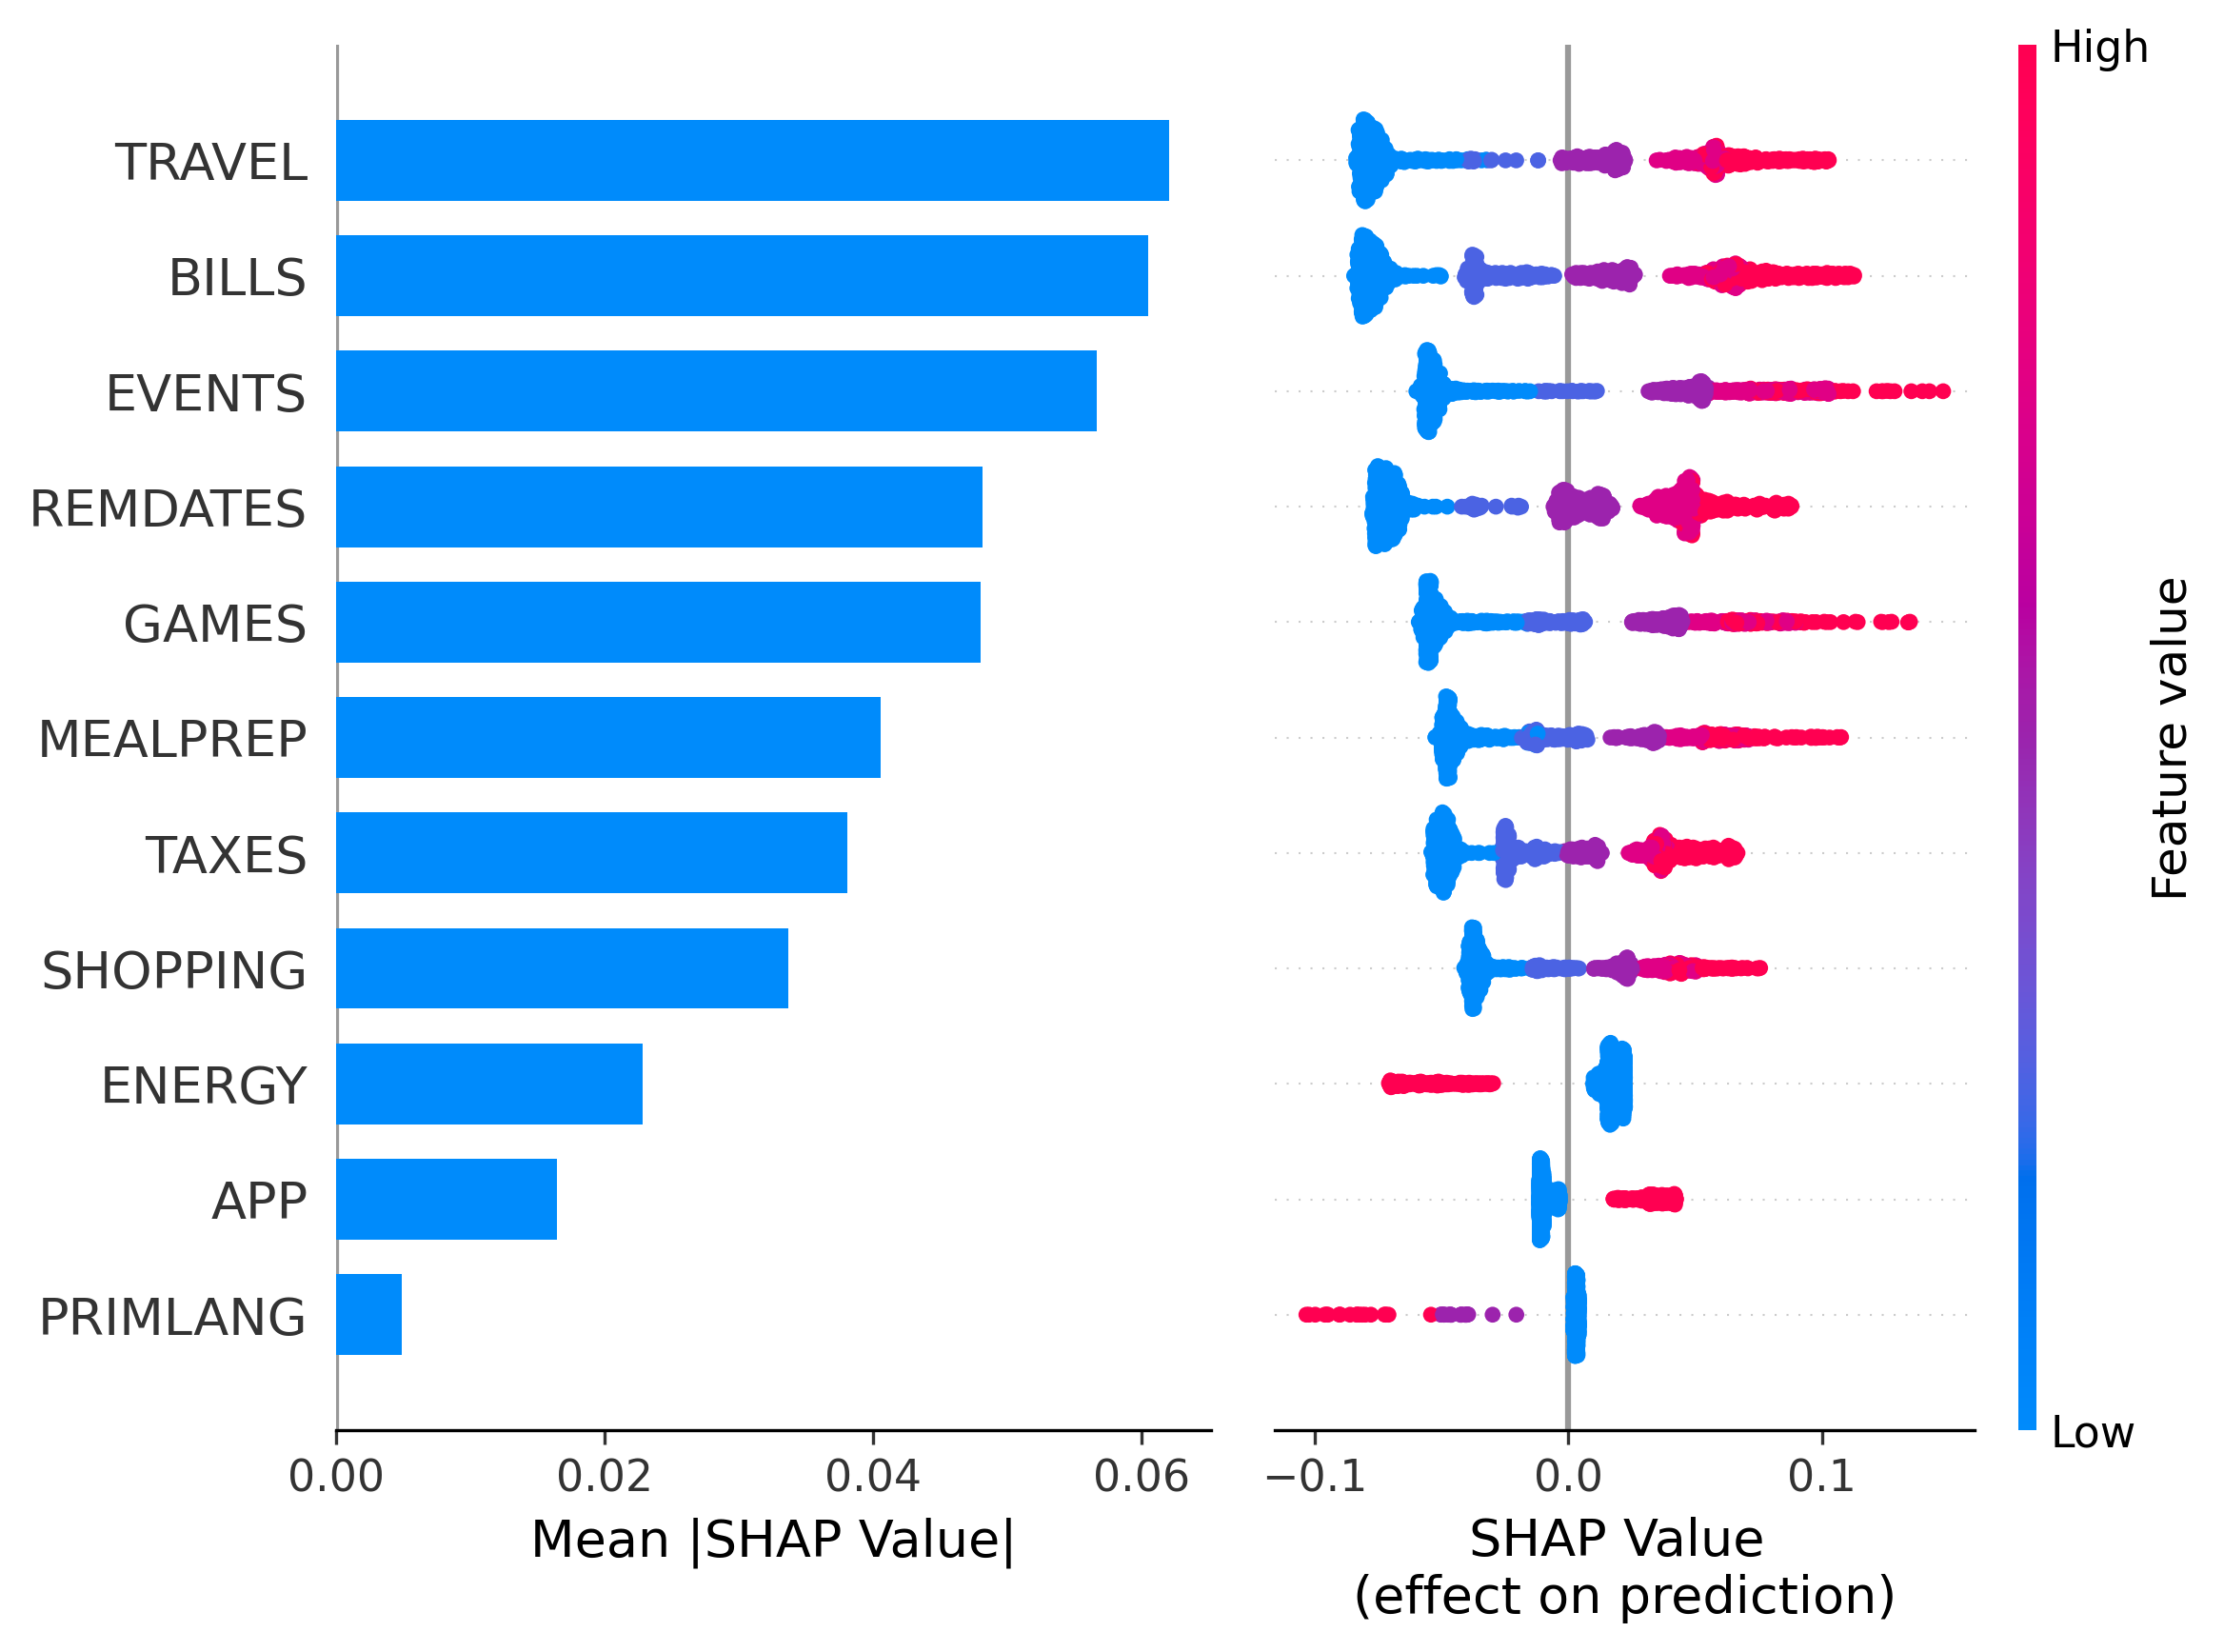
\includegraphics[width=\textwidth]{figures/appendix/dementia_classification_adni_shap_feature_importance.png}
        \caption*{(b) ADNI External Validation}
    \end{minipage}
    \caption{Feature importance with summary plot for the CIND vs. dementia classification task}
    \label{figure:summary-plot-task2-apdx}
\end{figure}

\begin{figure}[H]
    \centering
    \begin{minipage}{0.48\textwidth}
        \centering
        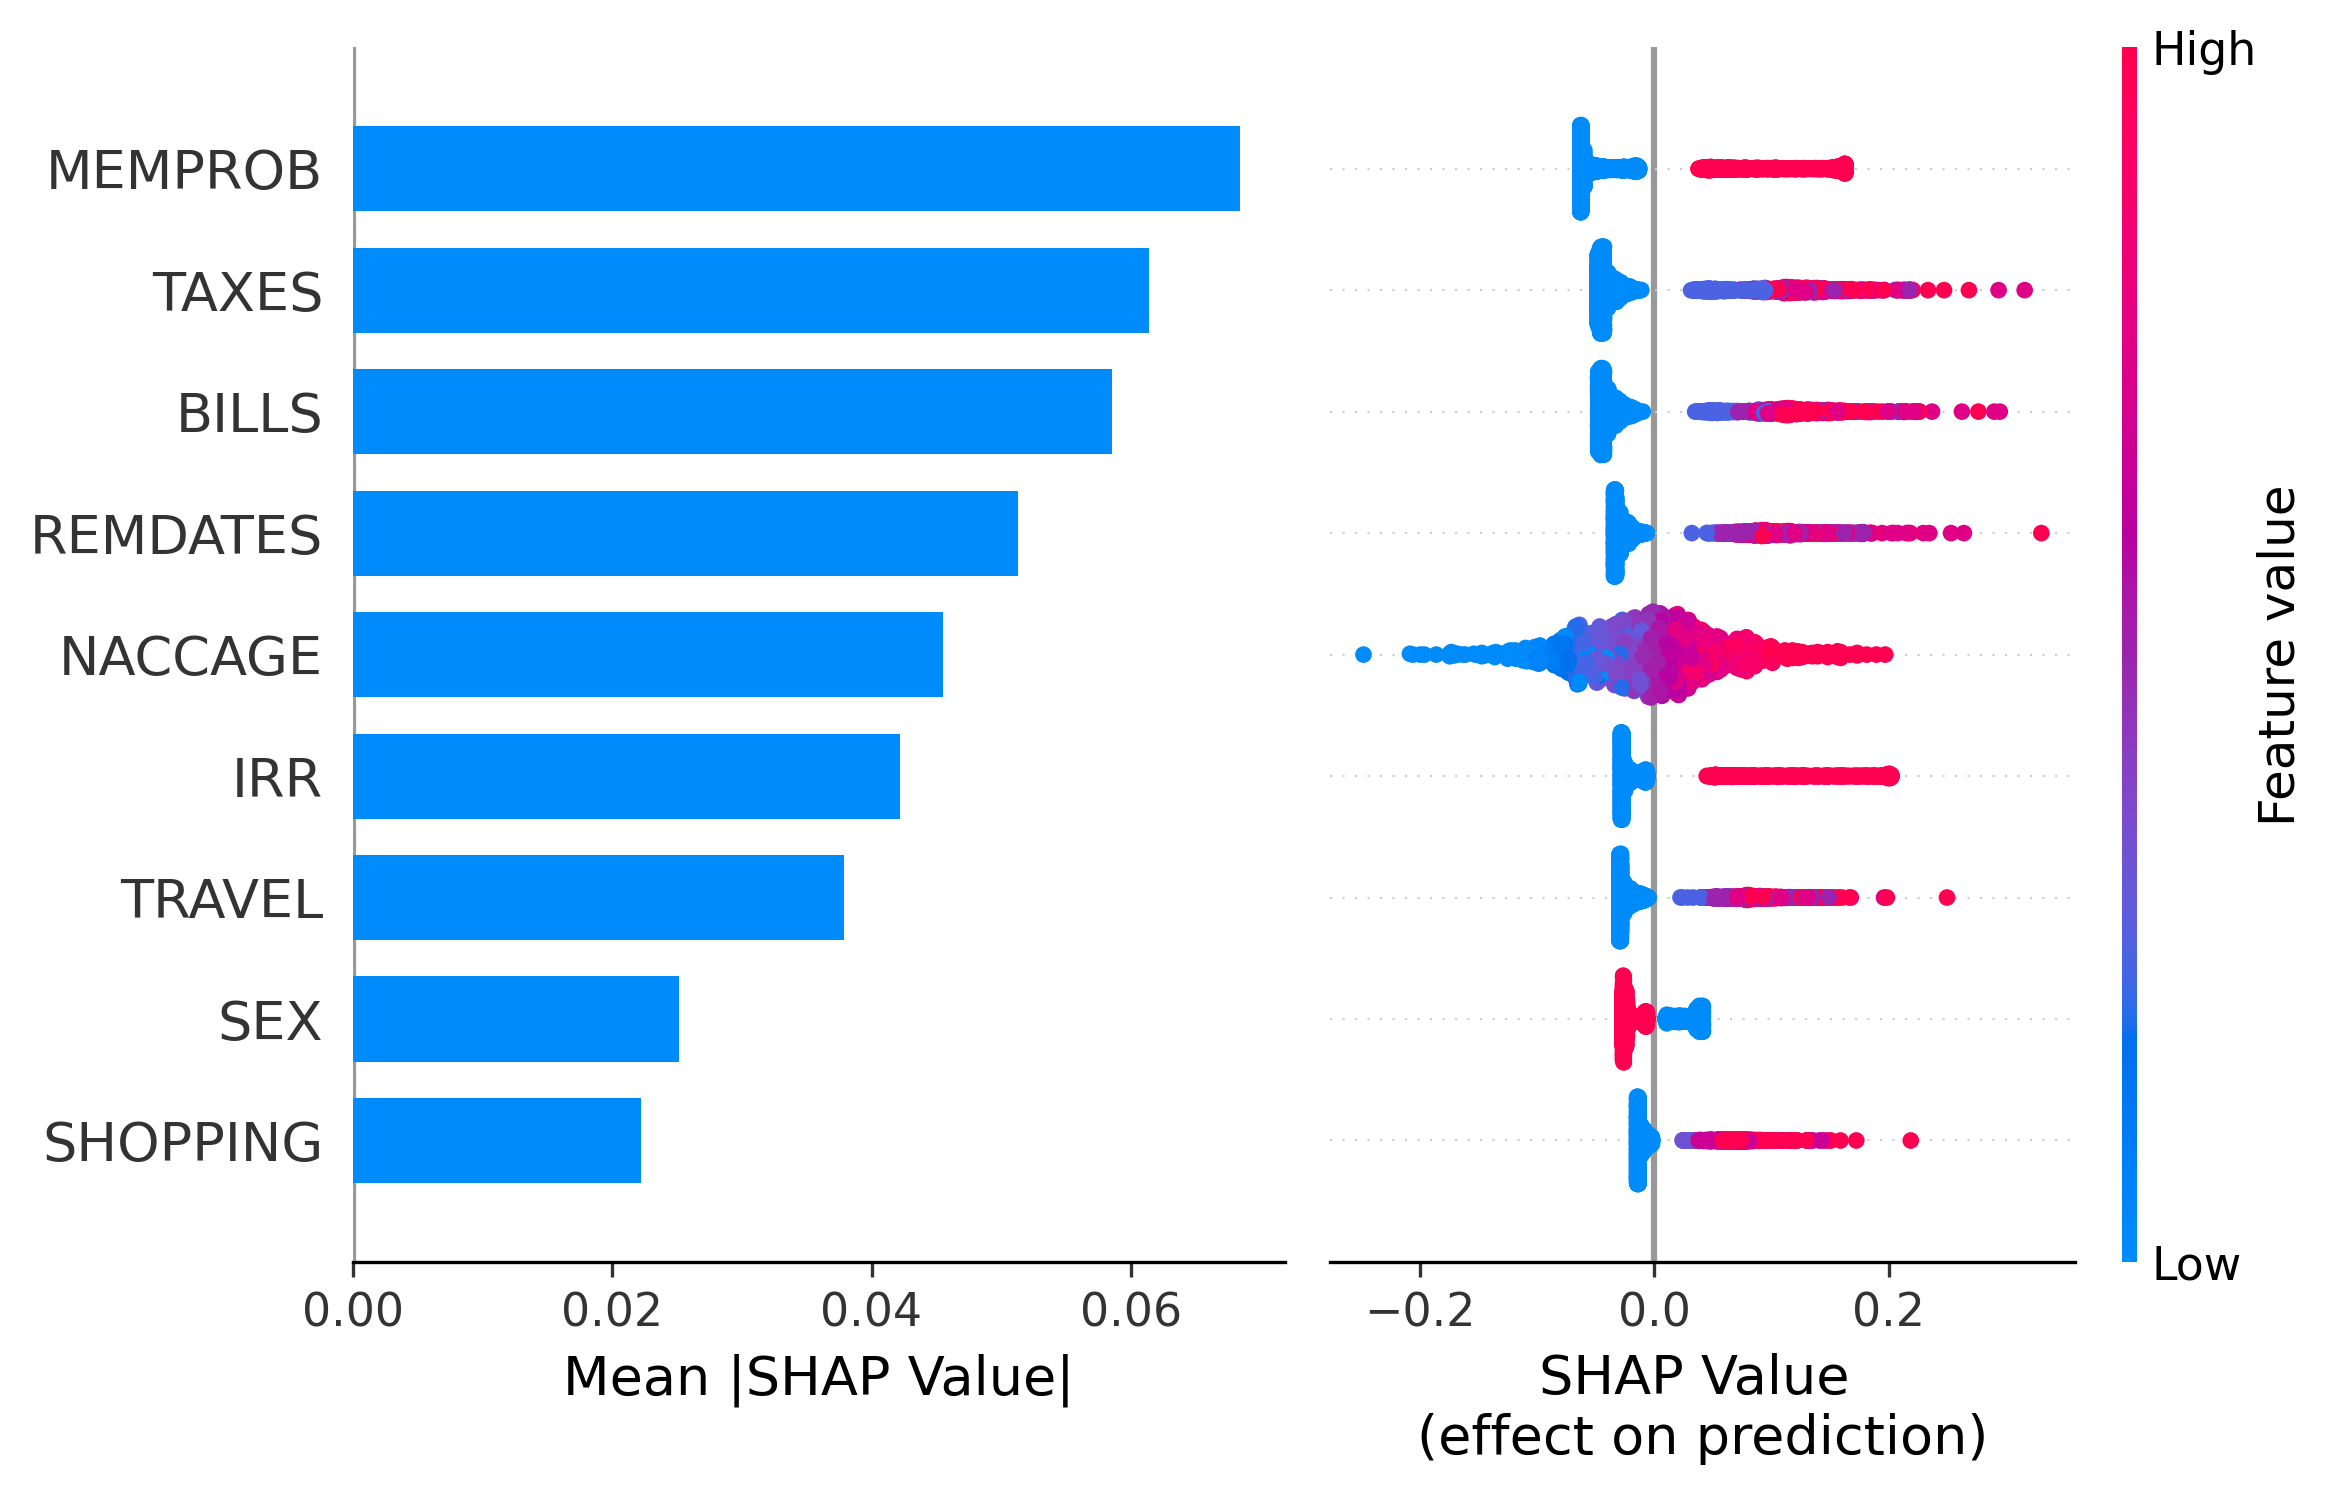
\includegraphics[width=\textwidth]{figures/appendix/impaired_prediction_nacc_shap_feature_importance.png}
        \caption*{(a)  NACC cross-center validation}
    \end{minipage}
    \begin{minipage}{0.48\textwidth}
        \centering
        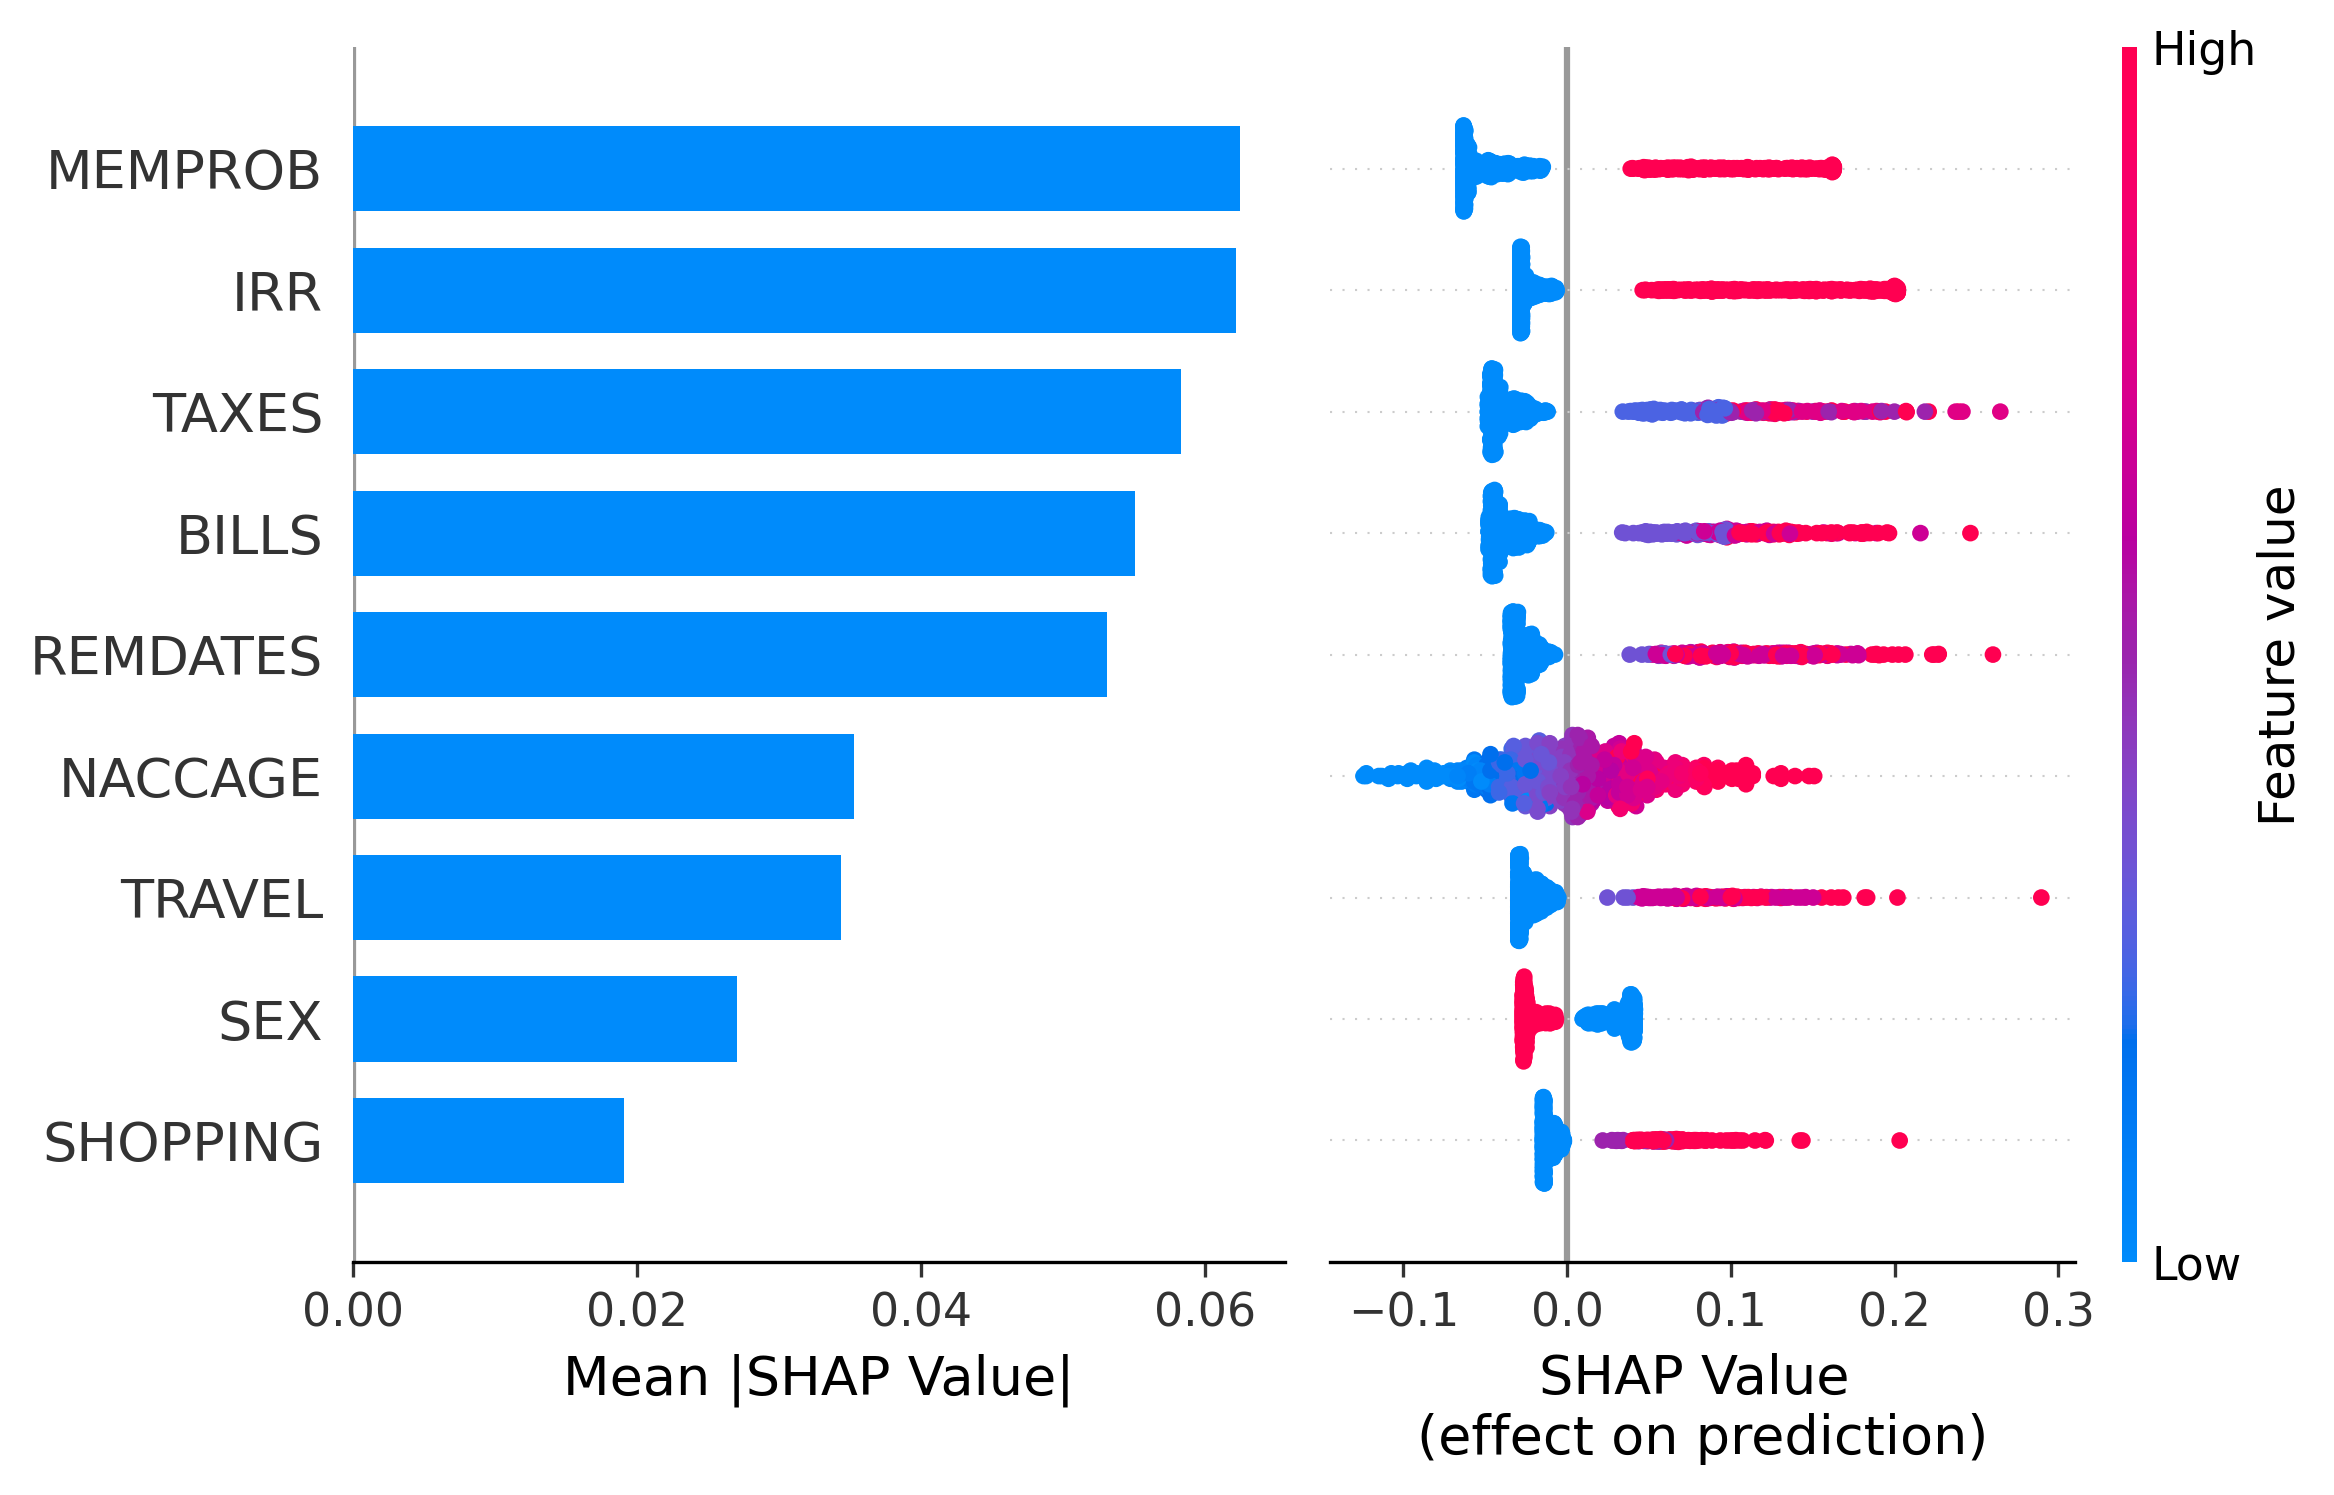
\includegraphics[width=\textwidth]{figures/appendix/impaired_prediction_adni_shap_feature_importance.png}
        \caption*{(b) ADNI External Validation}
    \end{minipage}
    \caption{Feature importance with summary plot for the feature NC vs. CI prediction task}
    \label{figure:summary-plot-task3-apdx}
\end{figure}

\begin{figure}[H]
    \centering
    \begin{minipage}{0.48\textwidth}
        \centering
        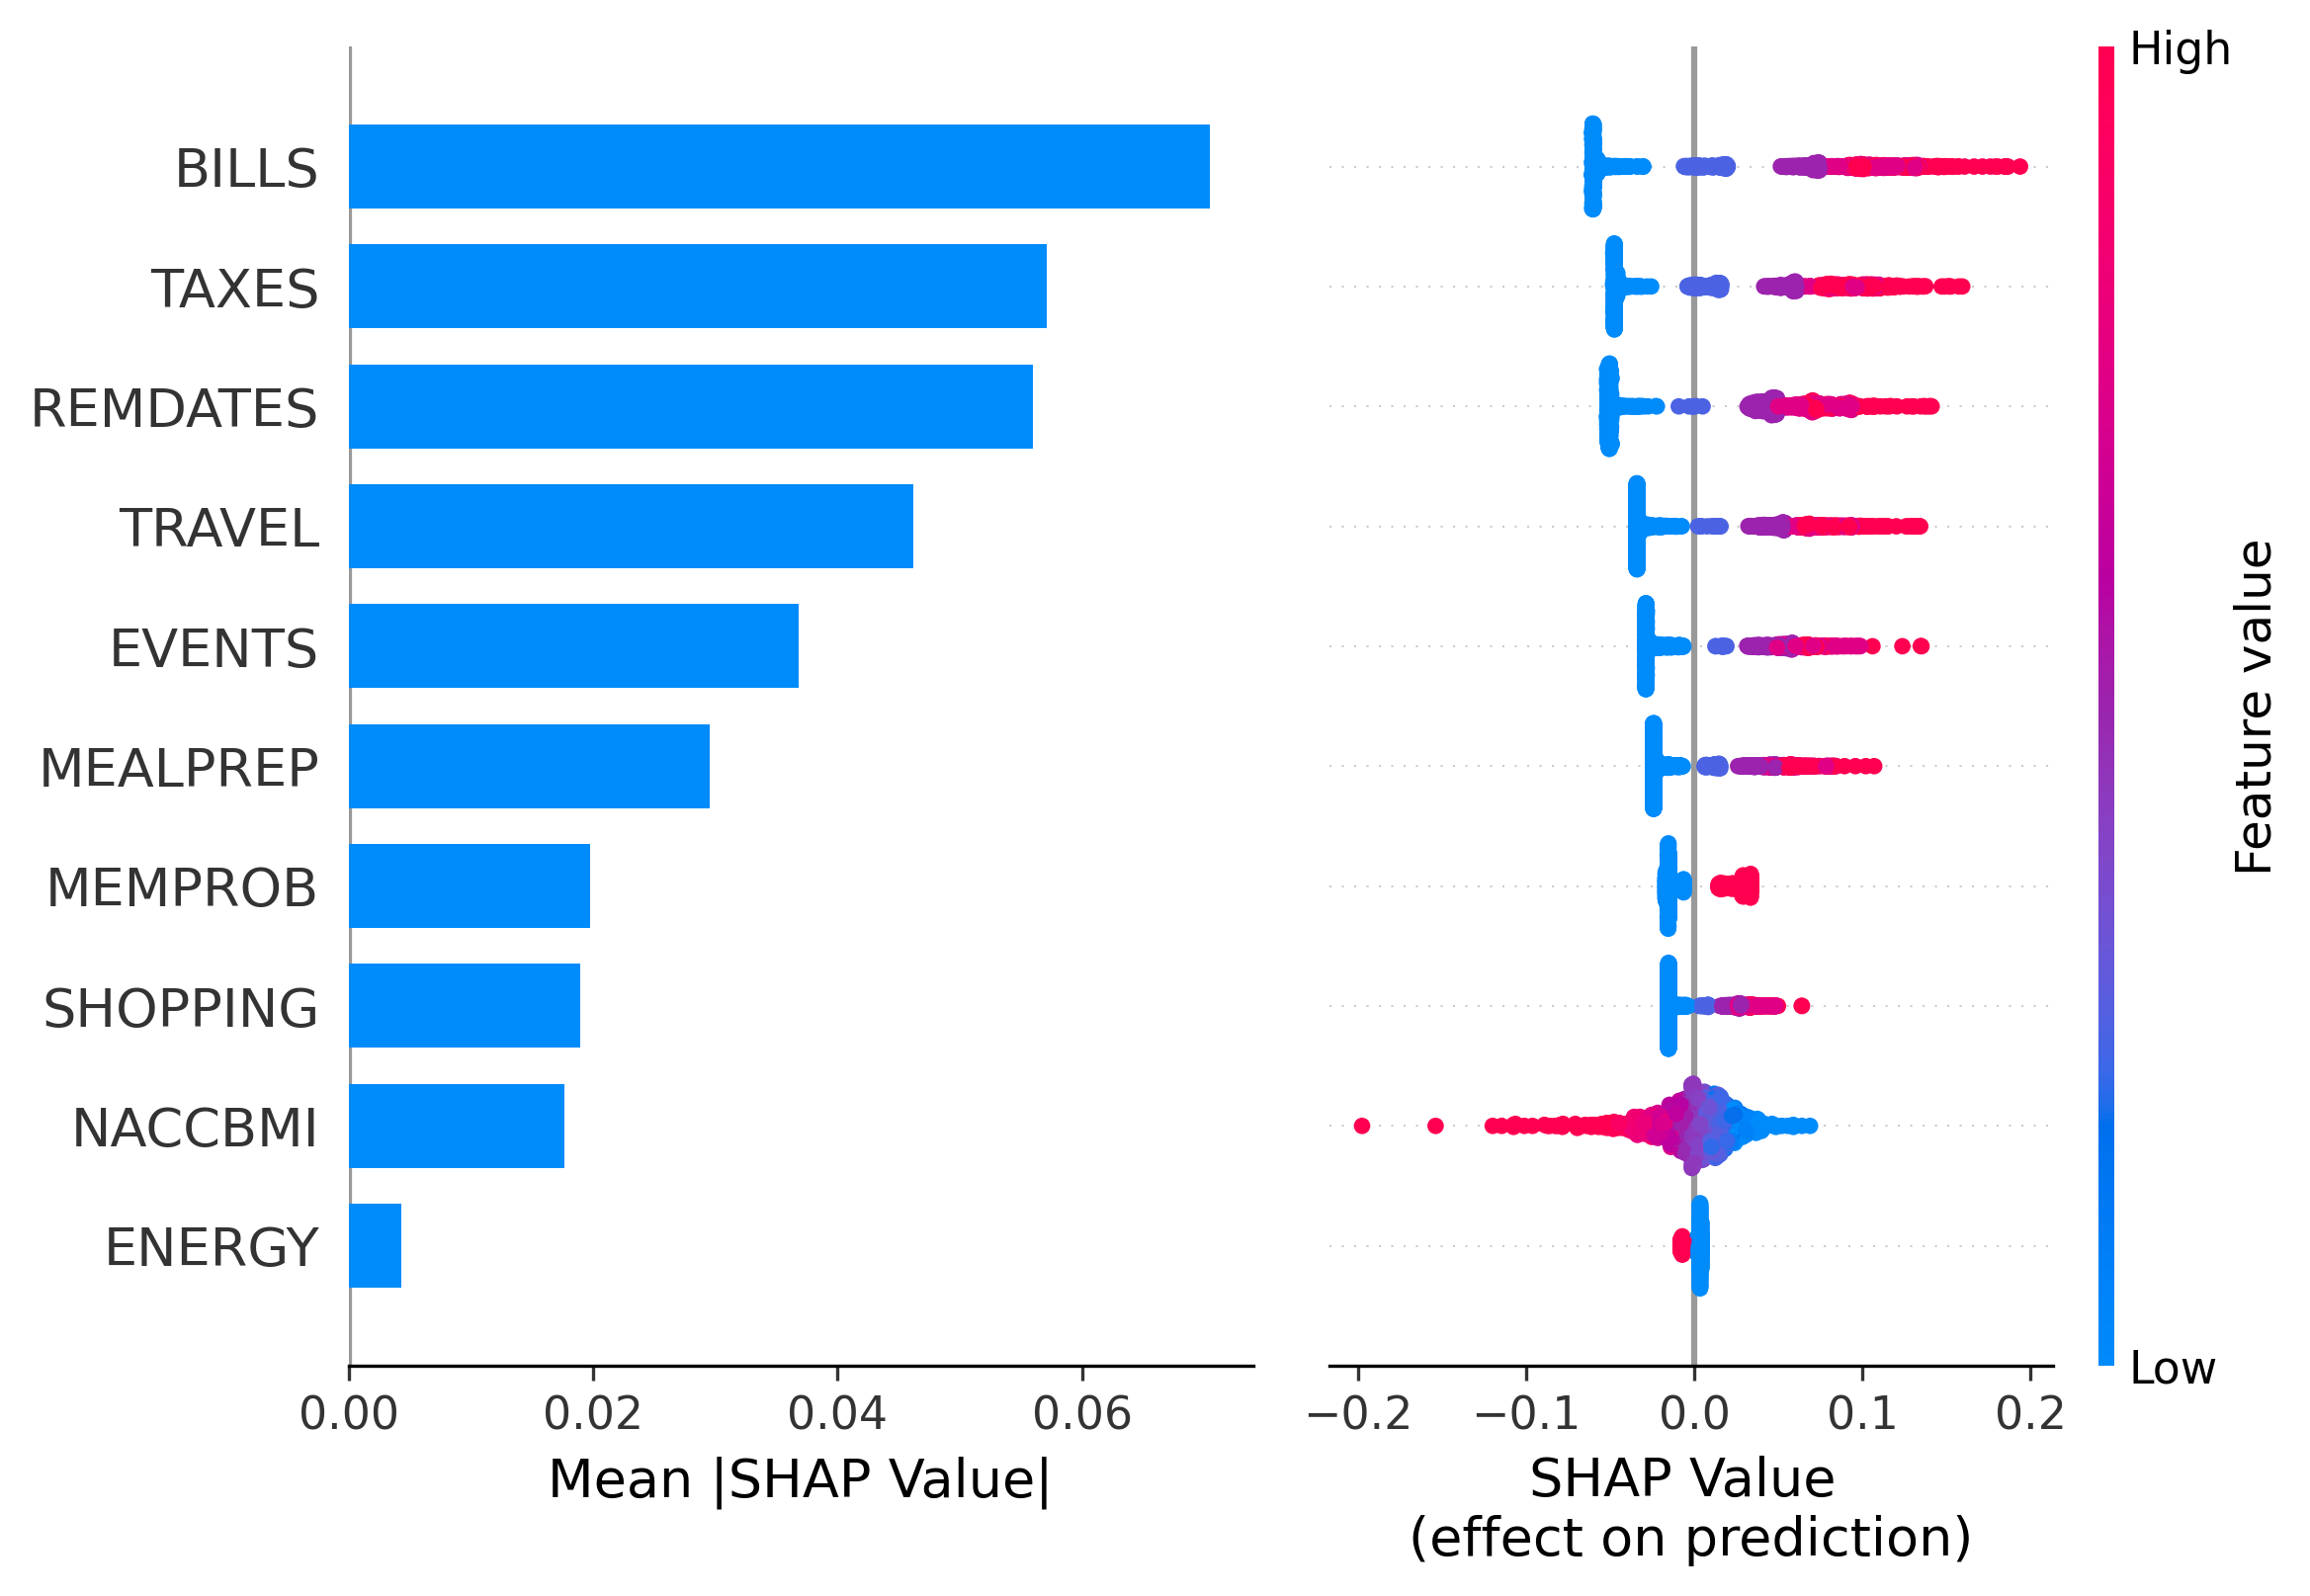
\includegraphics[width=\textwidth]{figures/appendix/dementia_prediction_nacc_shap_feature_importance.png}
        \caption*{(a)  NACC cross-center validation}
    \end{minipage}
    \begin{minipage}{0.48\textwidth}
        \centering
        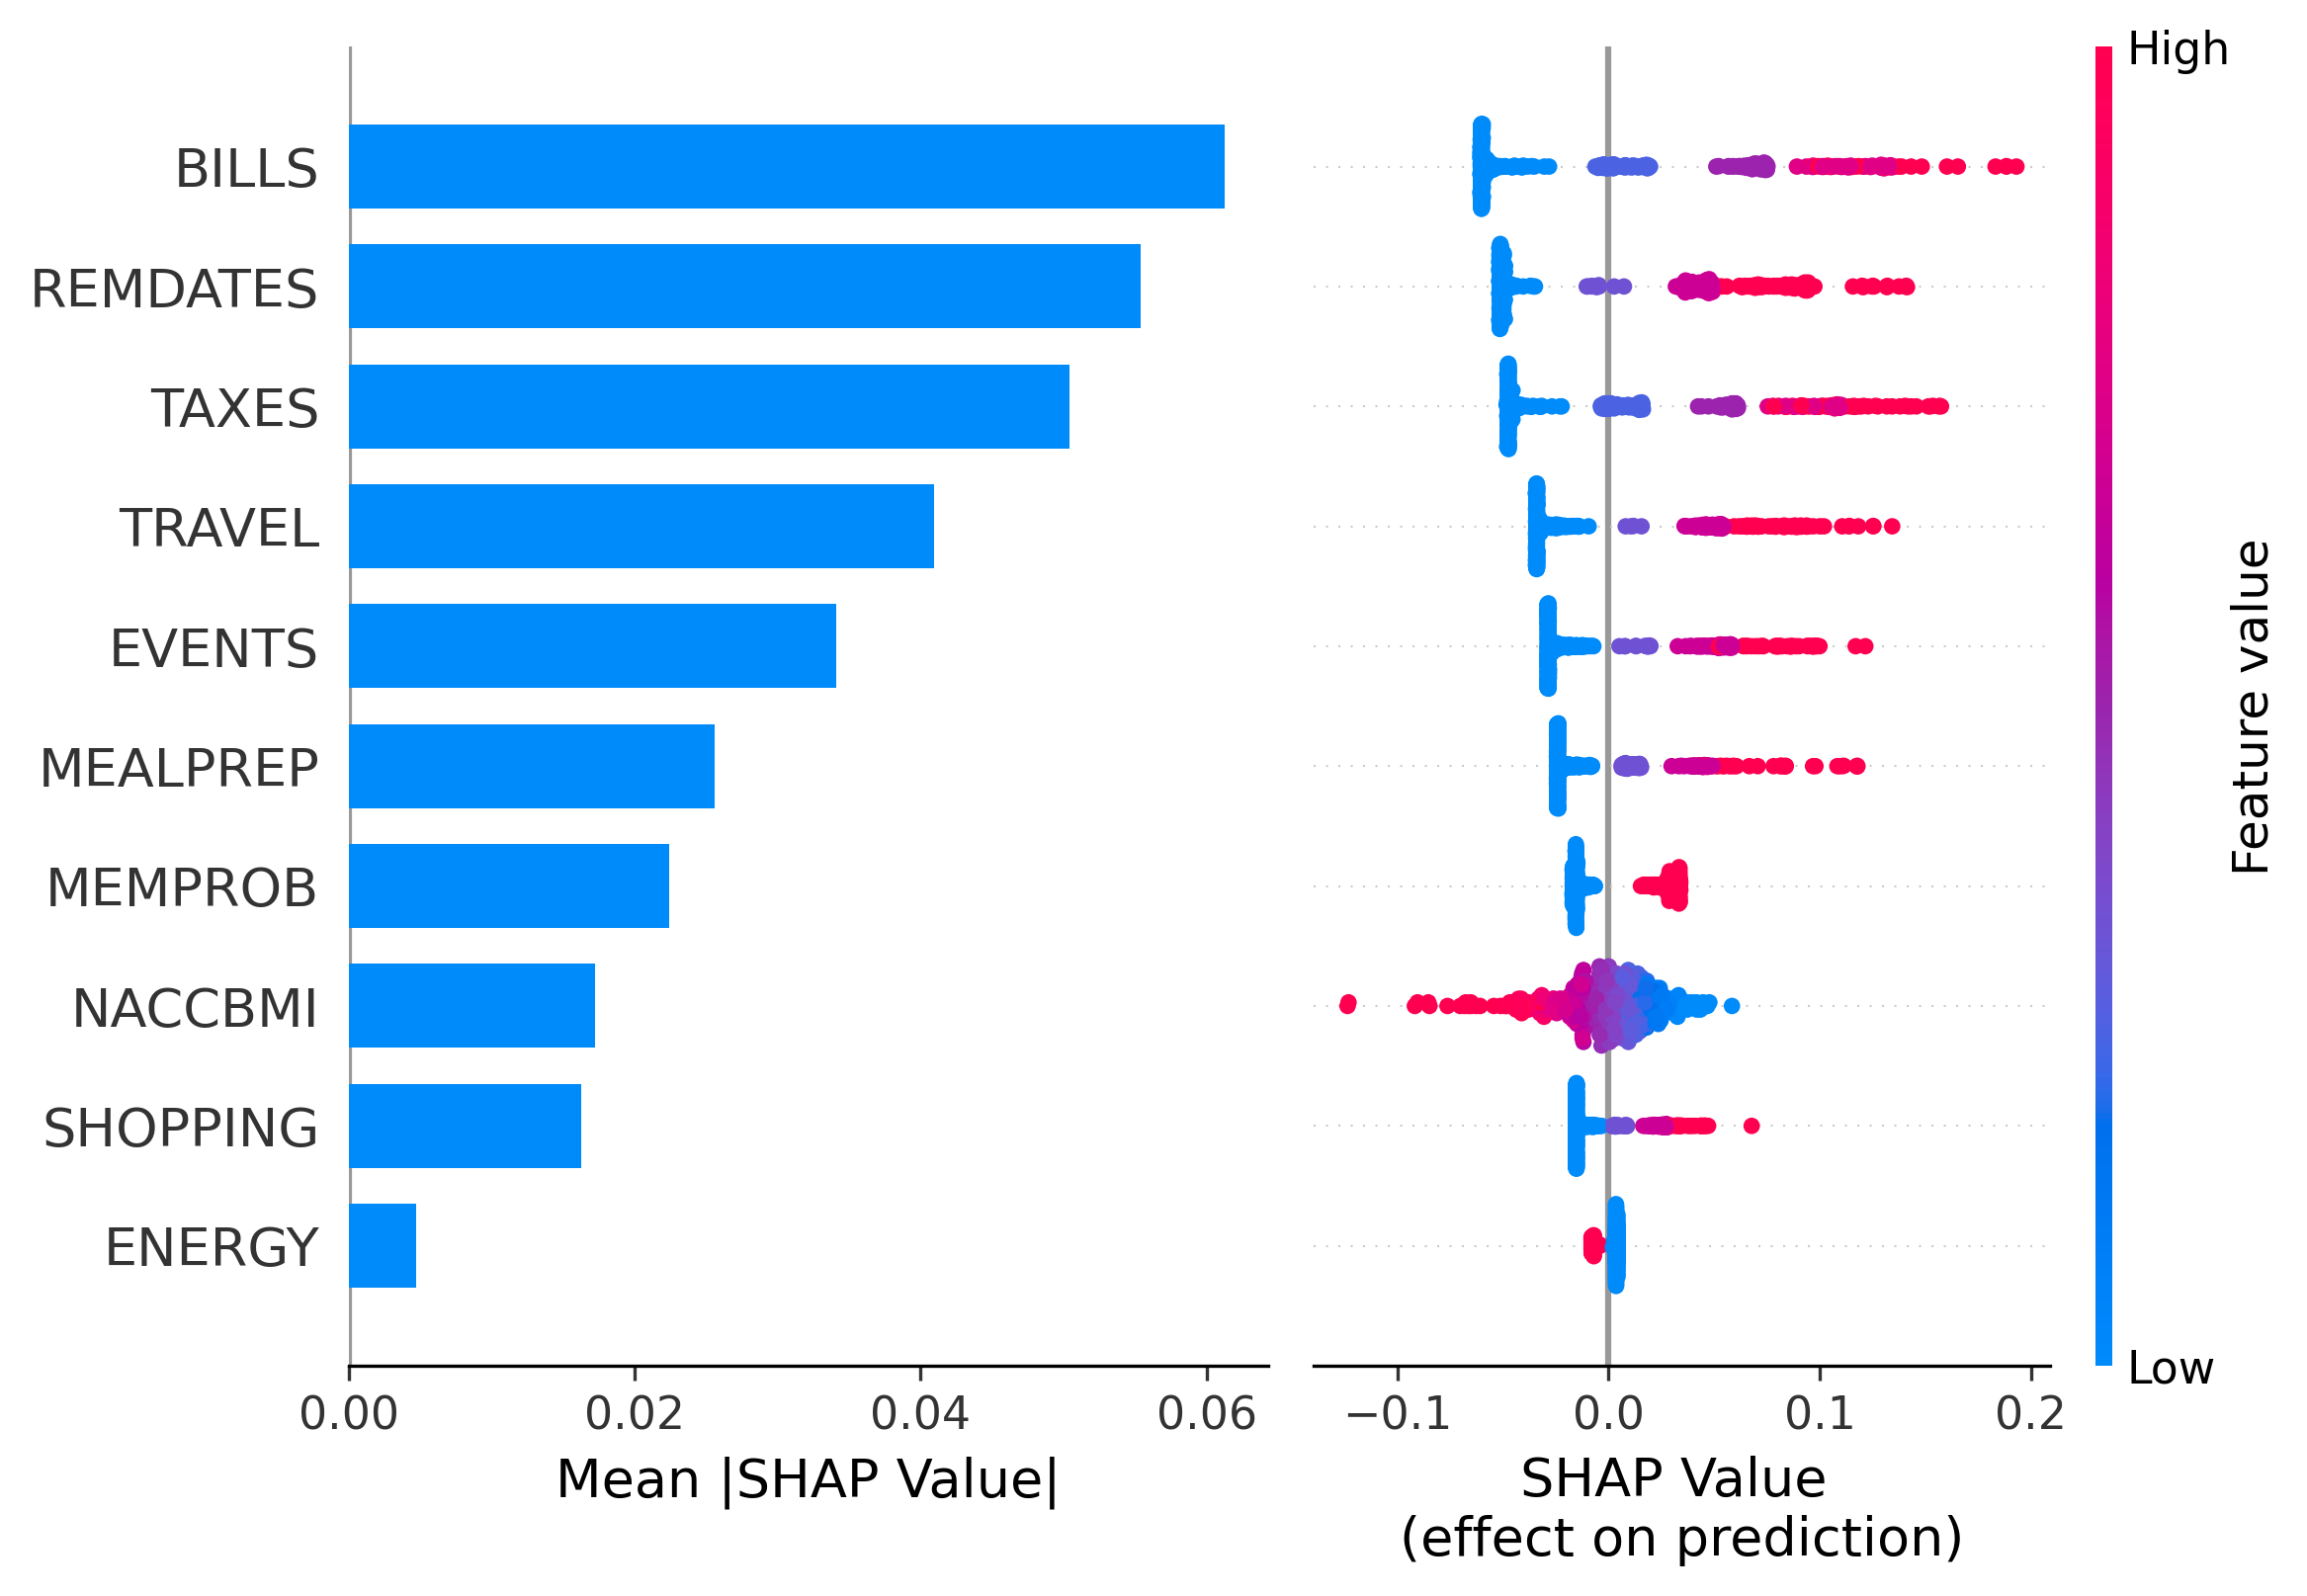
\includegraphics[width=\textwidth]{figures/appendix/dementia_prediction_adni_shap_feature_importance.png}
        \caption*{(b) ADNI External Validation}
    \end{minipage}
    \caption{Feature importance with summary plot for the feature CIND vs. dementia prediction task}
    \label{figure:summary-plot-task4-apdx}
\end{figure}

\begin{figure}[H]
    \centering
    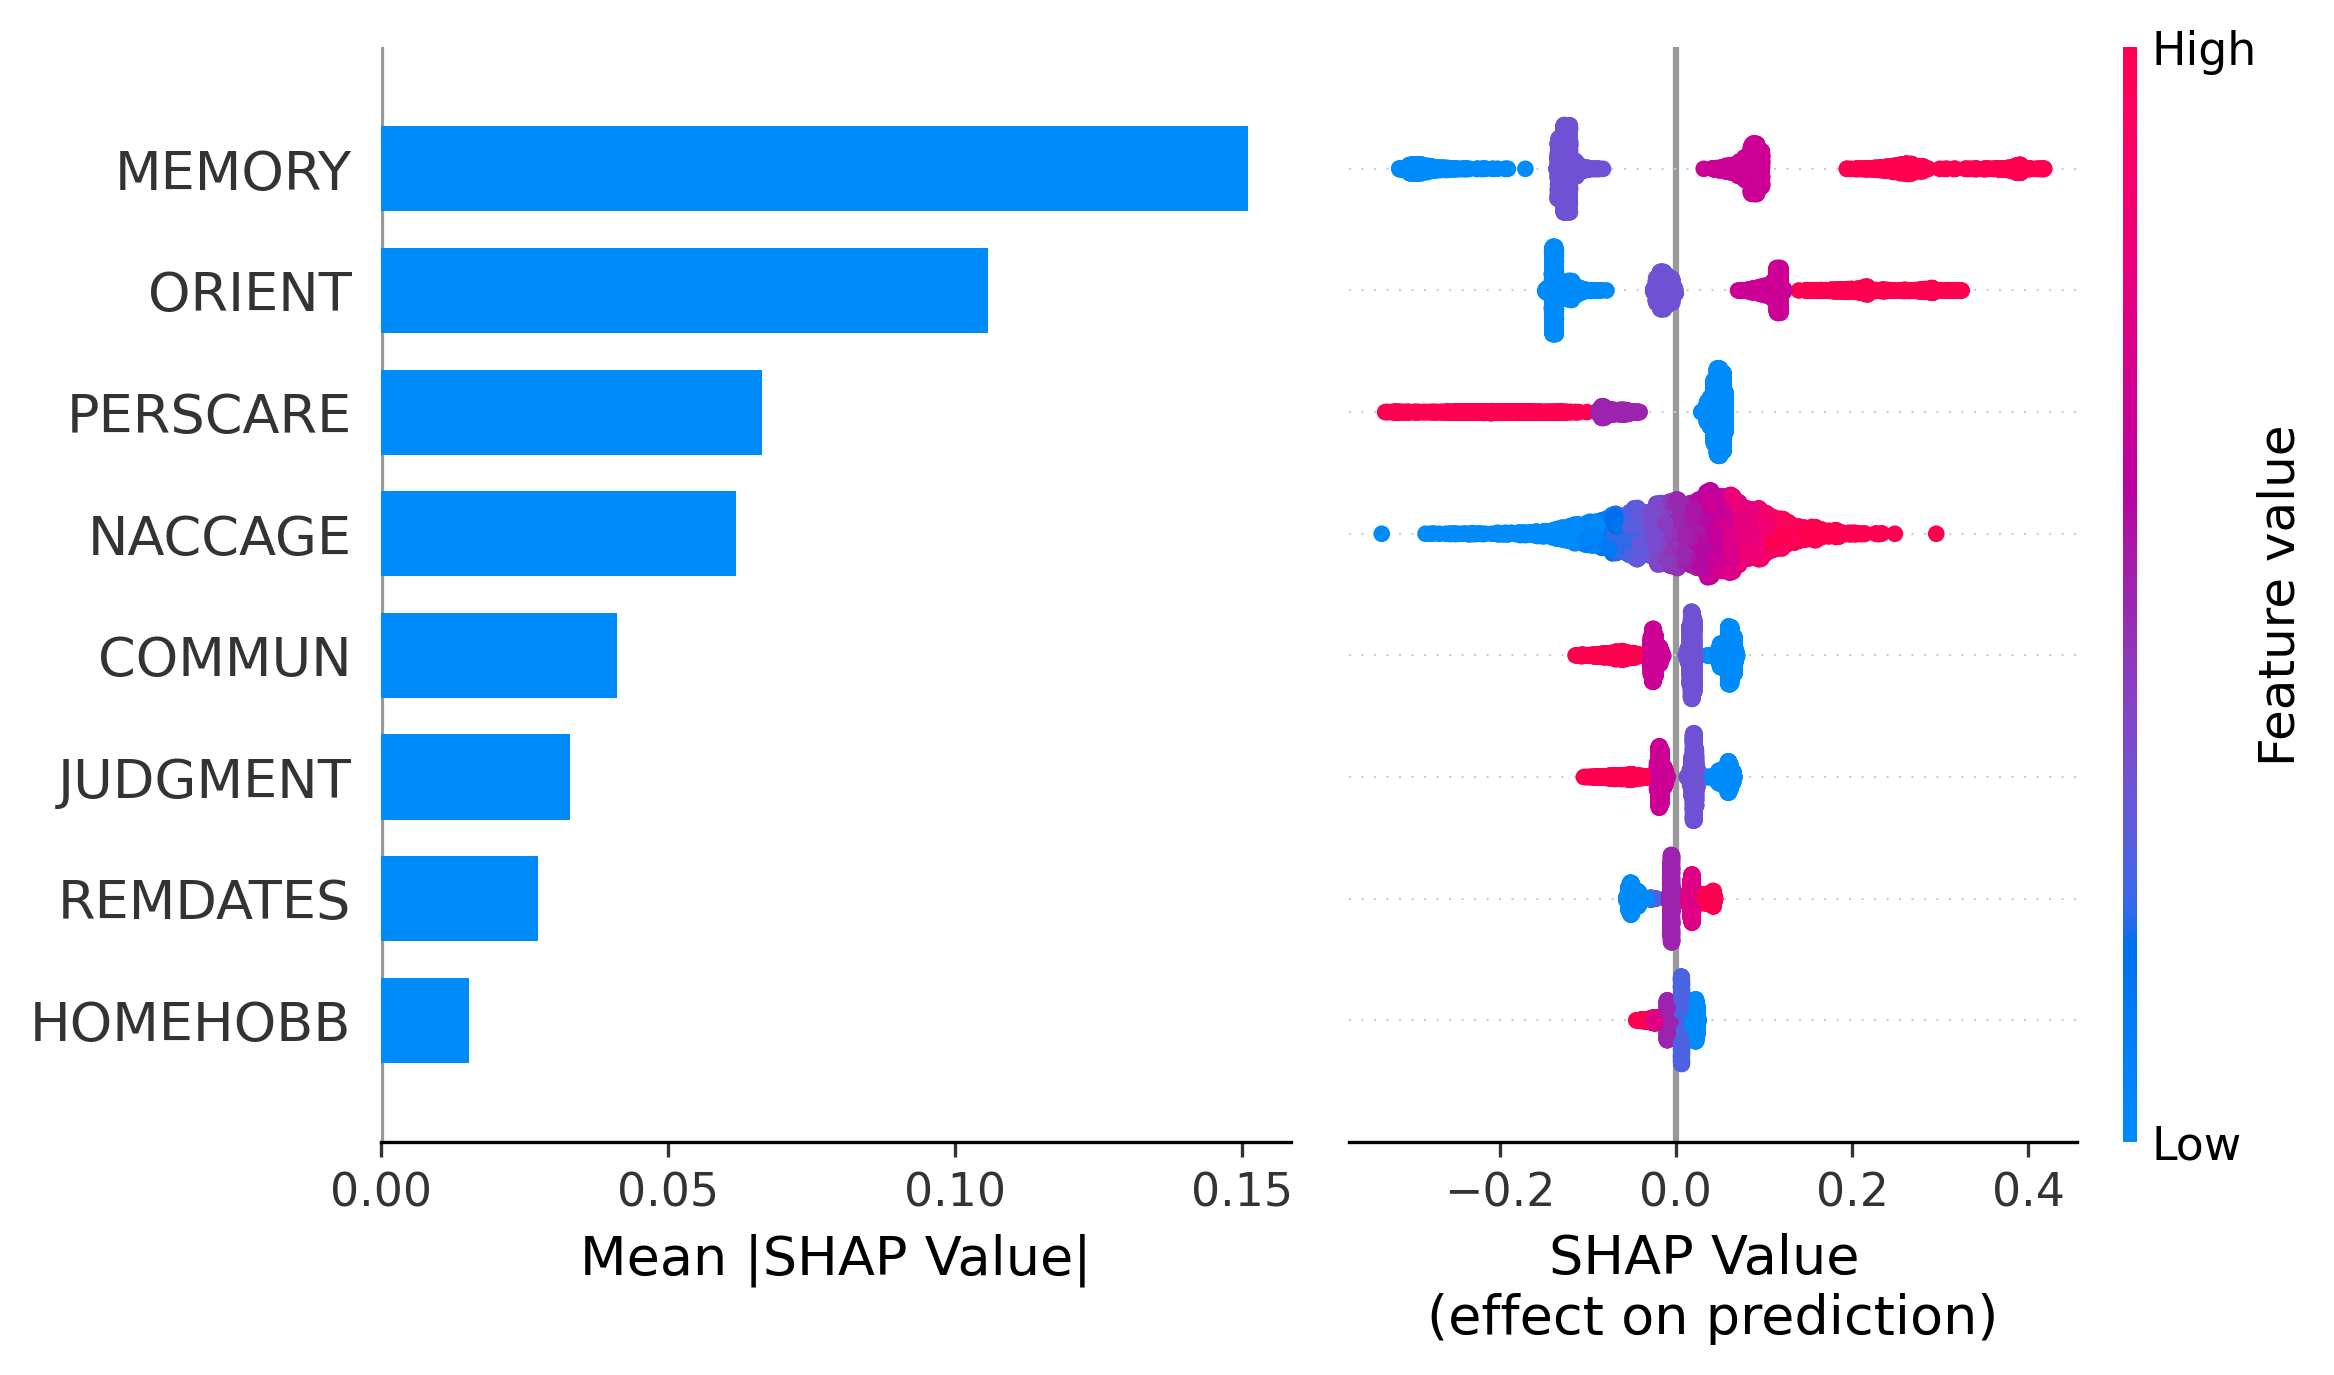
\includegraphics[width=0.7\textwidth]{figures/appendix/type_classification_nacc_shap_feature_importance.png}
    \caption{Feature importance with summary plot in the NACC cross-center validation for the AD vs. non-AD classification task}
    \label{figure:summary-plot-task5-apdx}
\end{figure}

% ----------------------------------------------------

\begin{figure}[H]
    \centering
    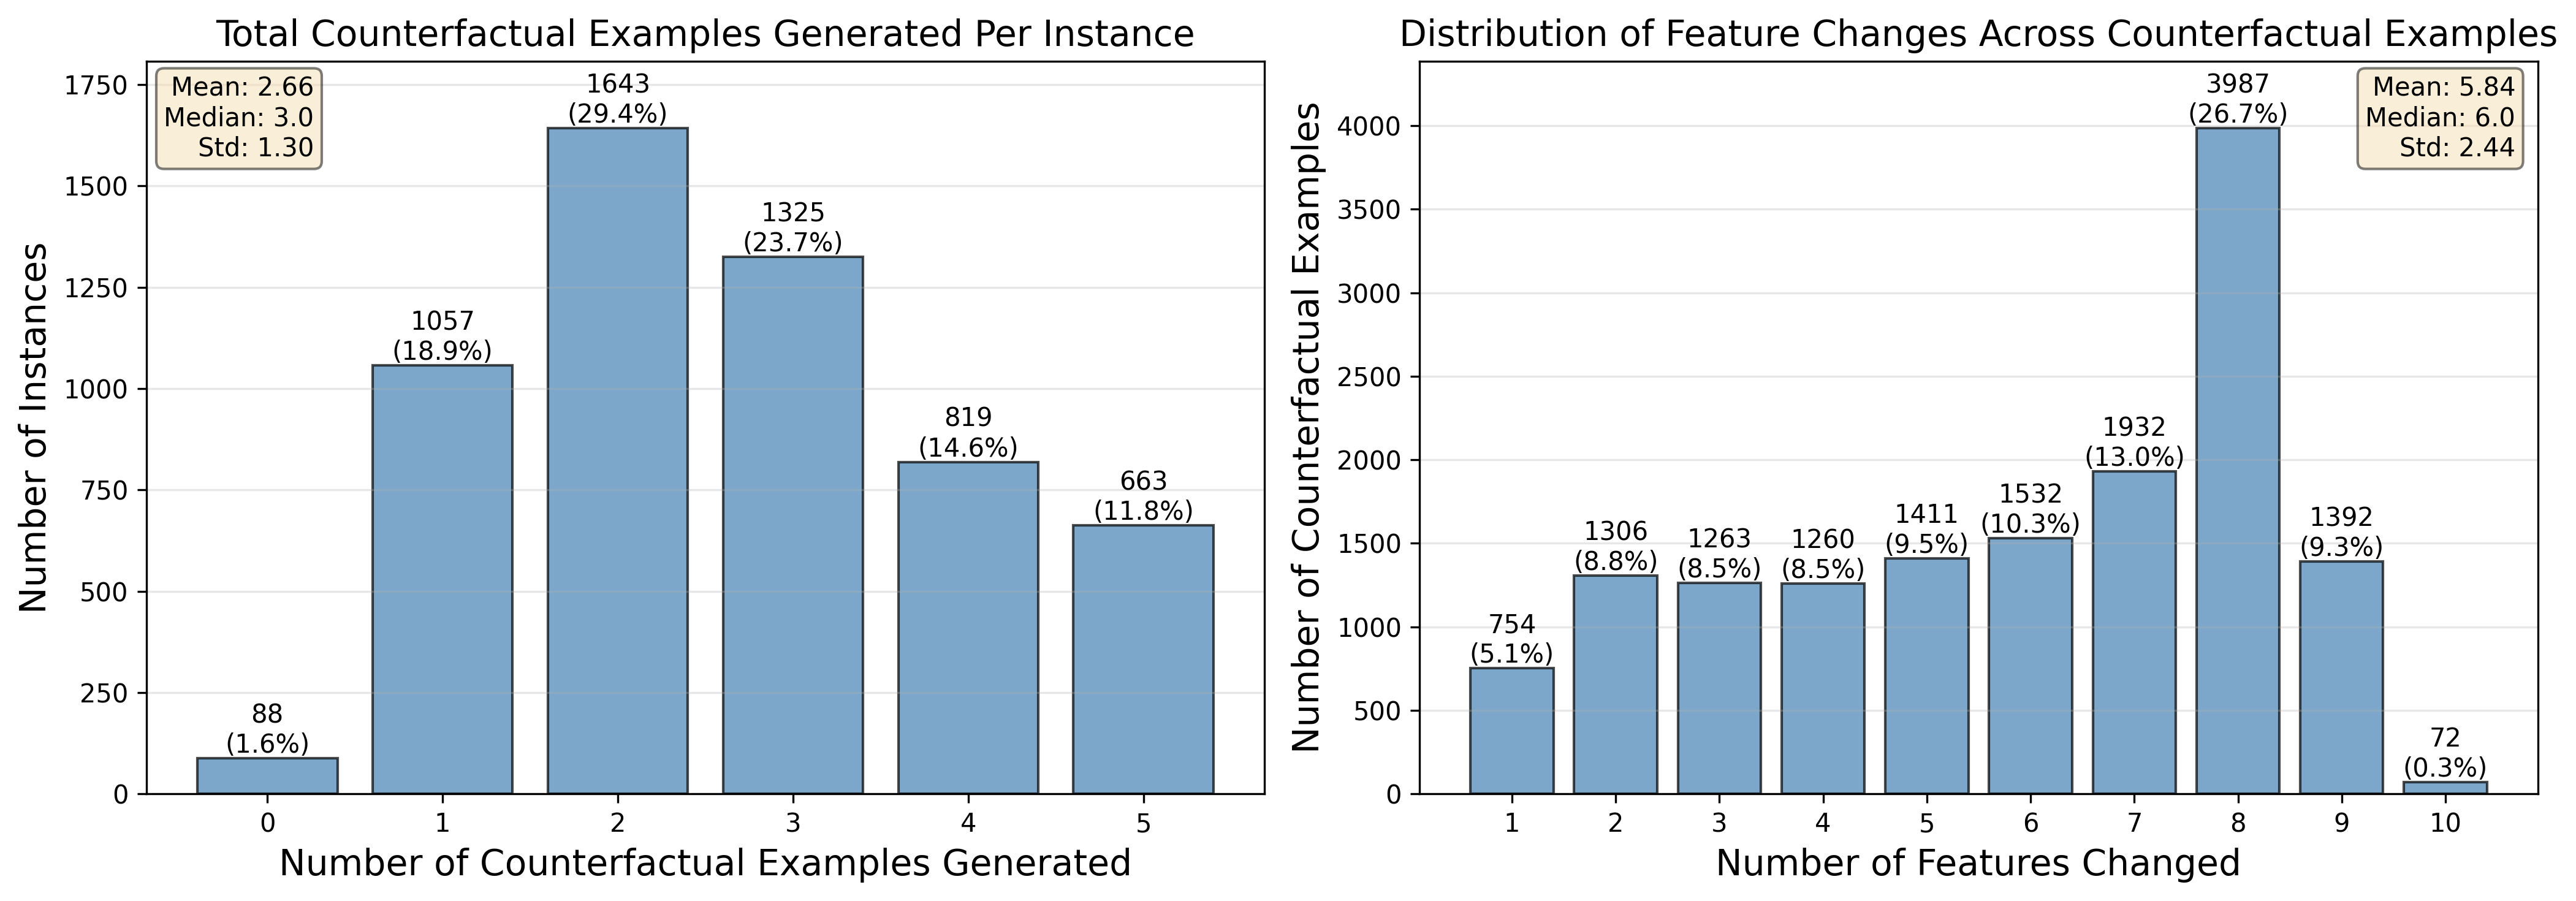
\includegraphics[width=\textwidth]{figures/appendix/impaired_classification_nacc_kdtree_dice_stats.png}
    \caption{Summary of generated counterfactual examples in the NACC cross-center validation for the NC vs. CI classification task}
    \label{figure:dice-nacc-task1-apdx}
\end{figure}

\begin{figure}[H]
    \centering
    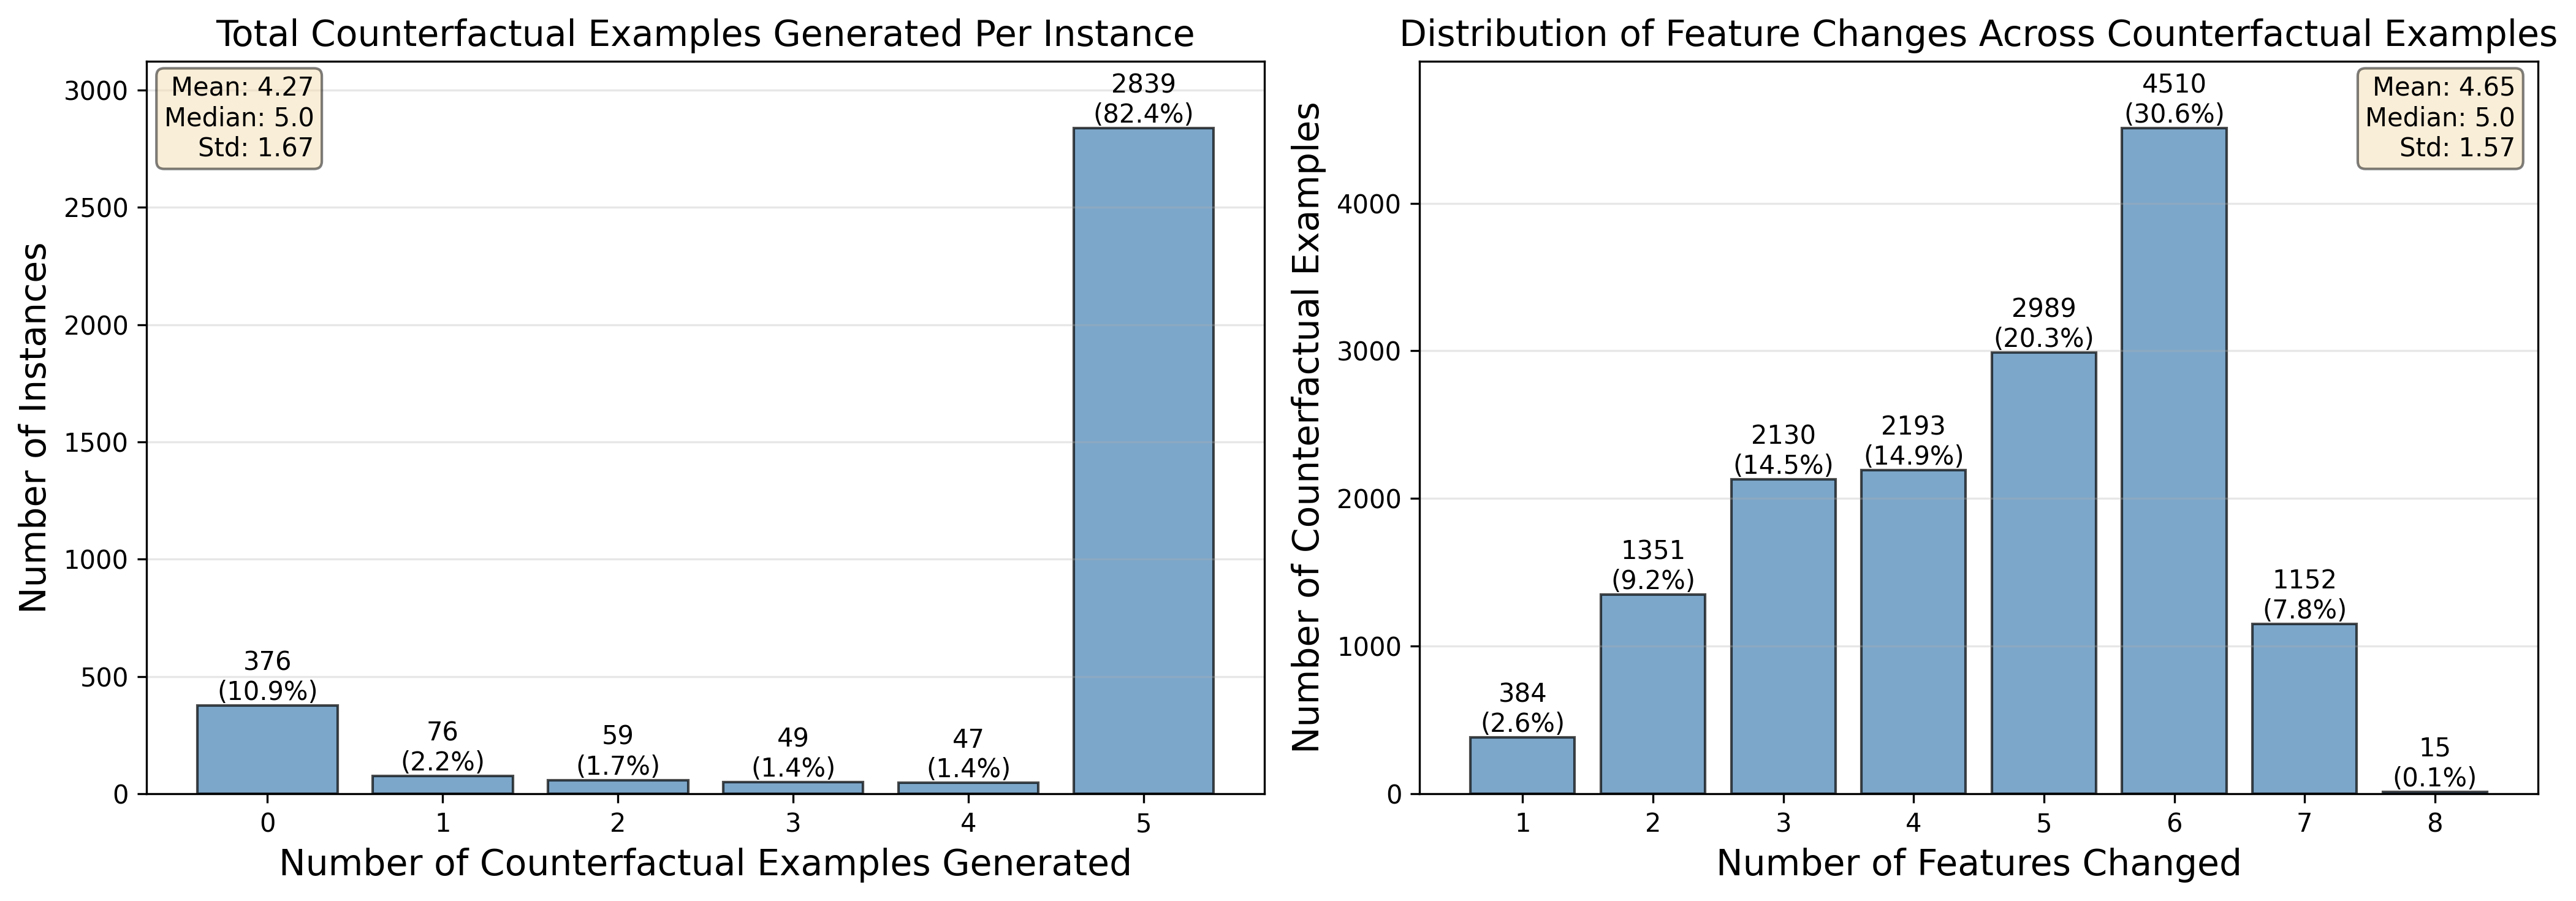
\includegraphics[width=\textwidth]{figures/appendix/dementia_classification_nacc_kdtree_dice_stats.png}
    \caption{Summary of generated counterfactual examples in the NACC cross-center validation for the CIND vs. dementia classification task}
    \label{figure:dice-nacc-task2-apdx}
\end{figure}

\begin{figure}[H]
    \centering
    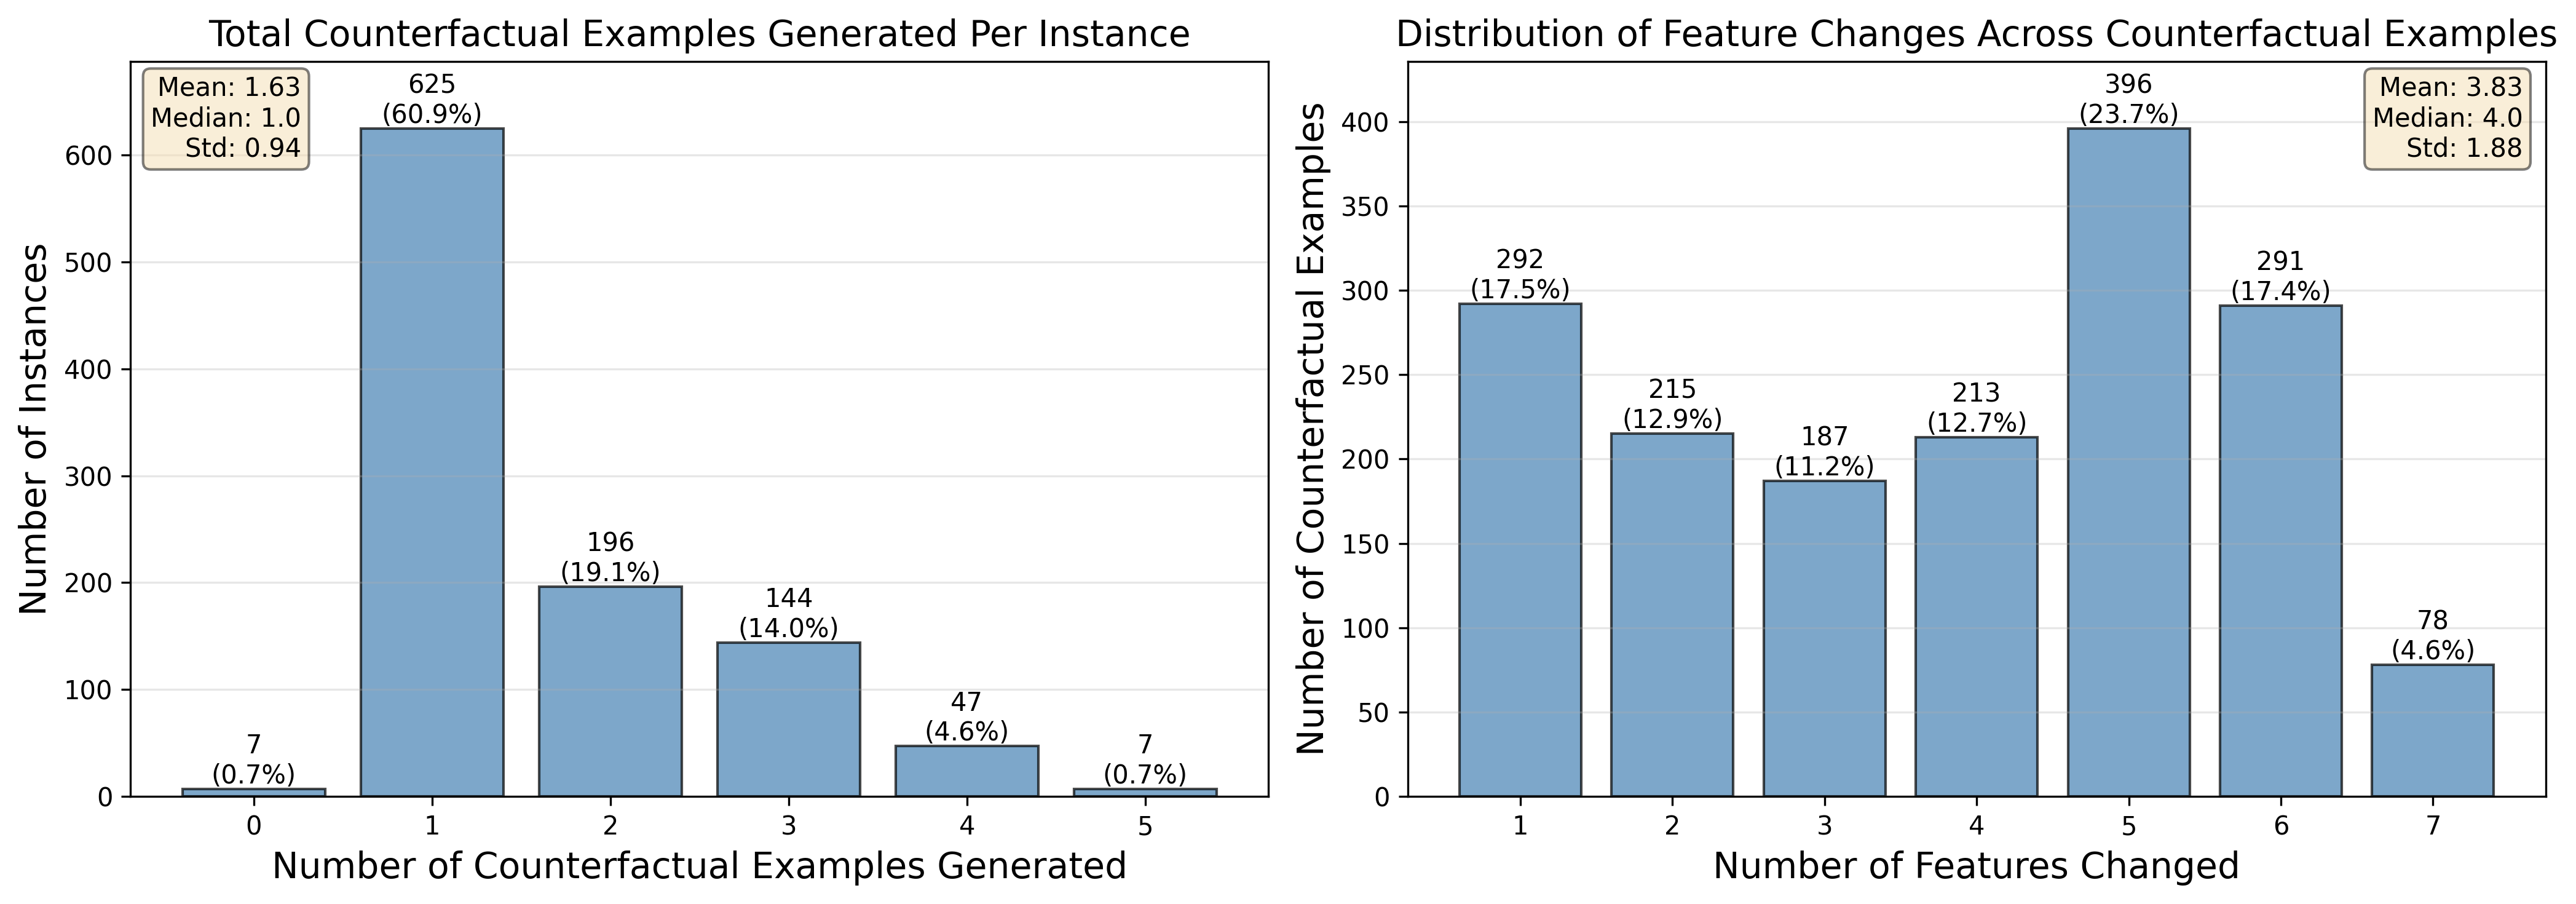
\includegraphics[width=\textwidth]{figures/appendix/impaired_prediction_nacc_kdtree_dice_stats.png}
    \caption{Summary of generated counterfactual examples in the NACC cross-center validation for the future NC vs. CI prediction task}
    \label{figure:dice-nacc-task3-apdx}
\end{figure}

\begin{figure}[H]
    \centering
    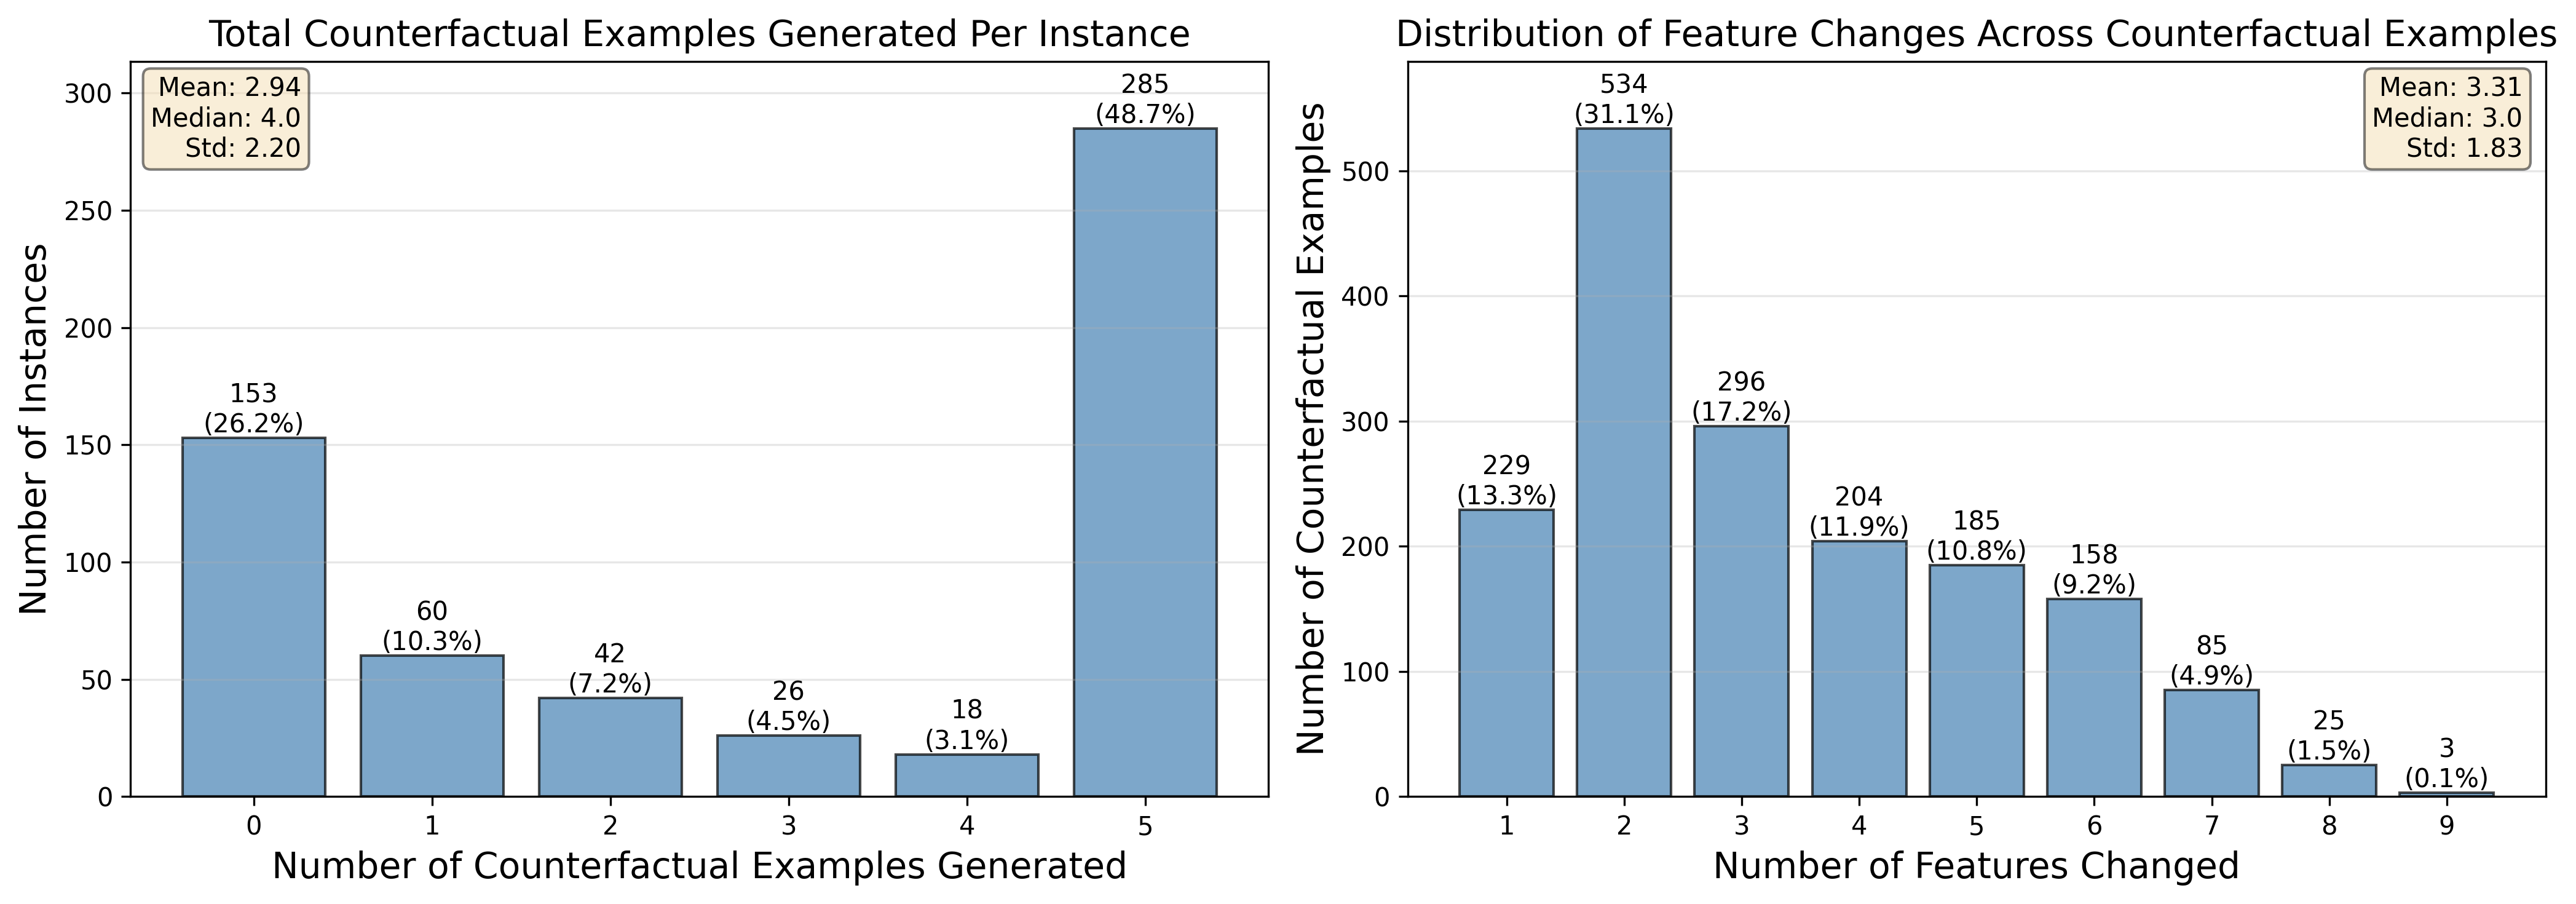
\includegraphics[width=\textwidth]{figures/appendix/dementia_prediction_nacc_random_dice_stats.png}
    \caption{Summary of generated counterfactual examples in the NACC cross-center validation for the future CIND vs.dementia prediction task}
    \label{figure:dice-nacc-task4-apdx}
\end{figure}

% ----------------------------------------------------

\begin{table}[H]
    \centering
    \caption{An illustration of counterfactual examples generated for a random subject classified as cognitive impairment (CI) to reverse the estimated outcome to normal cognition (NC)}
    \begin{tabular}{|c|c|c|c|c|}
    \hline
        \textbf{Feature} & \textbf{Original} & \textbf{CFE1} & \textbf{CFE2} & \textbf{CFE3} \\ \hline
        NACCAGE & 61 & ~ & ~ & ~ \\ \hline
        SEX & Male & ~ & ~ & ~ \\ \hline
        ANX & Yes & ~ & No & No \\ \hline
        MEMPROB & No & ~ & ~ & ~ \\ \hline
        BILLS & Normal & ~ & ~ & ~ \\ \hline
        TAXES & Normal & ~ & ~ & ~ \\ \hline
        SHOPPING & Normal & ~ & ~ & ~ \\ \hline
        GAMES & Normal & ~ & ~ & ~ \\ \hline
        EVENTS & Normal & ~ & ~ & ~ \\ \hline
        PAYATTN & Has difficulty & Normal & Normal & Normal \\ \hline
        REMDATES & Has difficulty & Normal & ~ & Normal \\ \hline
        TRAVEL & Has difficulty & Normal & Normal & ~ \\ \hline
        Outcome & CI & NC & NC & NC \\ \hline
    \multicolumn{5}{p{280pt}}{\footnotesize Empty cells indicate no change in feature values. Refer to Table~\ref{table:feature-details} for more details about the features. CFE: counterfactual examples.}
    \end{tabular}
    \label{table:cfe-adni-task1-apdx}
\end{table}

\begin{table}[H]
    \centering
    \caption{An illustration of counterfactual examples generated for a random subject classified as dementia to reverse the estimated outcome to cognitive impairment but not dementia (\acrshort{CIND})}
    \begin{tabular}{|c|c|c|c|c|}
    \hline
        \textbf{Feature} & \textbf{Original} & \textbf{CFE1} & \textbf{CFE2} & \textbf{CFE3} \\ \hline
        APP & Yes & ~ & ~ & No \\ \hline
        ENERGY & Yes & ~ & ~ & ~ \\ \hline
        BILLS & Requires assistance & Normal & ~ & Has difficulty \\ \hline
        TAXES & Dependent & ~ & Has difficulty & ~ \\ \hline
        SHOPPING & Normal & ~ & ~ & ~ \\ \hline
        GAMES & Normal & ~ & ~ & ~ \\ \hline
        MEALPREP & Normal & ~ & ~ & ~ \\ \hline
        EVENTS & Has difficulty & ~ & ~ & ~ \\ \hline
        REMDATES & Has difficulty & ~ & ~ & ~ \\ \hline
        TRAVEL & Dependent & Normal & Normal & Normal \\ \hline
        PRIMLANG & English & ~ & ~ & ~ \\ \hline
        Outcome & dementia & CIND & CIND & CIND \\ \hline
    \multicolumn{5}{p{350pt}}{\footnotesize Empty cells indicate no change in feature values. Refer to Table~\ref{table:feature-details} for more details about the features. CFE: counterfactual examples.}
    \end{tabular}
    \label{table:cfe-adni-task2-apdx}
\end{table}

\begin{table}[H]
    \centering
    \caption{An illustration of counterfactual examples generated for a random subject with a future risk of cognitive impairment (CI) to reverse the estimated outcome to normal cognition (NC)}
    \begin{tabular}{|c|c|c|c|c|}
    \hline
        \textbf{Feature} & \textbf{Original} & \textbf{CFE1} & \textbf{CFE2} & \textbf{CFE3} \\ \hline
        NACCAGE & 64 & ~ & ~ & ~ \\ \hline
        SEX & Female & ~ & ~ & ~ \\ \hline
        IRR & Yes & ~ & No & No \\ \hline
        MEMPROB & No & ~ & ~ & ~ \\ \hline
        BILLS & Normal & ~ & ~ & ~ \\ \hline
        TAXES & Normal & ~ & ~ & ~ \\ \hline
        SHOPPING & Normal & ~ & ~ & ~ \\ \hline
        REMDATES & Requires assistance & Normal & Normal & Has difficulty \\ \hline
        TRAVEL & Has difficulty & Normal & ~ & Normal \\ \hline
        Outcome & CI & NC & NC & NC \\ \hline
    \multicolumn{5}{p{350pt}}{\footnotesize Empty cells indicate no change in feature values. Refer to Table~\ref{table:feature-details} for more details about the features. CFE: counterfactual examples.}
    \end{tabular}
    \label{table:cfe-adni-task3-apdx}
\end{table}

\begin{table}[H]
    \centering
    \caption{An illustration of counterfactual examples generated for a random subject with a future risk of dementia to reverse the estimated outcome to cognitive impairment but not dementia (\acrshort{CIND})}
    \begin{tabular}{|c|c|c|c|c|}
    \hline
        \textbf{Feature} & \textbf{Original} & \textbf{CFE1} & \textbf{CFE2} & \textbf{CFE3} \\ \hline
        NACCBMI & 29.0 & ~ & ~ & 22.6 \\ \hline
        MEMPROB & Yes & No & ~ & ~ \\ \hline
        ENERGY & Yes & No & ~ & ~ \\ \hline
        BILLS & Normal & ~ & ~ & ~ \\ \hline
        TAXES & Has difficulty & ~ & ~ & Normal \\ \hline
        SHOPPING & Normal & ~ & ~ & ~ \\ \hline
        MEALPREP & Never did & ~ & ~ & ~ \\ \hline
        EVENTS & Normal & ~ & ~ & ~ \\ \hline
        REMDATES & Has difficulty & ~ & Normal & ~ \\ \hline
        TRAVEL & Normal & ~ & ~ & ~ \\ \hline
        Outcome & dementia & CIND & CIND & CIND \\ \hline
    \multicolumn{5}{p{280pt}}{\footnotesize Empty cells indicate no change in feature values. Refer to Table~\ref{table:feature-details} for more details about the features. CFE: counterfactual examples.}
    \end{tabular}
    \label{table:cfe-adni-task4-apdx}
\end{table}

\section{Summary of the Comparative Analysis with Existing Literature}\label{sec:compare-summary-apdx}
This section provides a summary of the comparison between this study and the reviewed studies discussed in Section~\ref{sec:performance-comparison}. The comparison in Table~\ref{table:compare-summary} is presented across the main dimensions of methodological quality that affect the reliability, the cost-effectiveness, and the clinical utility of the developed models.

\setlength{\tabcolsep}{4pt}
\begin{longtable}{|M{0.18\textwidth}|M{0.40\textwidth}|M{0.06\textwidth}|M{0.06\textwidth}|M{0.06\textwidth}|M{0.06\textwidth}|M{0.06\textwidth}|}
\caption{Summary of the comparative analysis between this study and the reviewed literature across the main dimensions of methodological quality}
\label{table:compare-summary} \\
\hline
\textbf{Study} & \textbf{Key Features} & \rh{External Validation} & \rh{Calibration / DCA} & \rh{Class Imbalance Handling} & \rh{Class Overlap Analysis} & \rh{Computational Cost} \\
\hline
\endfirsthead

\caption[]{Summary of the comparative analysis between this study and the reviewed literature, continued} \\
\hline
\textbf{Study} & \textbf{Key Features} & \rh{External Validation} & \rh{Calibration / DCA} & \rh{Class Imbalance Handling} & \rh{Class Overlap Analysis} & \rh{Computational Cost} \\
\hline
\endhead

\hline
\multicolumn{7}{r}{\textit{Continued on next page}} \\
\endfoot

\hline
\multicolumn{7}{p{\textwidth}}{\footnotesize ADL: activities of daily living; CDR: clinical dementia rating; DCA: decision curve analysis; EHR: electronic health records; IADL: instrumental activities of daily living; MMSE: Mini-Mental State Examination. The check mark (\yesmark) indicates that the dimension was addressed or reported, the cross (\nomark) indicates that it was not, and the dash (\partialmark) indicates a partial case. In the external validation column, a partial case refers to a prospective validation on the same cohort rather than a separate external dataset, while in the computational cost column it refers to a study that reported only the computation time of the model.} \\
\endlastfoot

\textbf{This Study} & Demographic, functional (IADL); CDR for subtype & \yesmark & \yesmark & \yesmark & \yesmark & \yesmark \\
\hline
\cite{Gurevich2017Neuropsychological} & Demographic, neuropsychological tests & \nomark & \nomark & \nomark & \nomark & \nomark \\
\hline
\cite{Ben2020Predicting} & EHR: diagnoses, medications, notes & \nomark & \nomark & \nomark & \nomark & \nomark \\
\hline
\cite{Park2020Machine} & Claims and EHR: labs, diagnoses, medications & \nomark & \nomark & \nomark & \nomark & \nomark \\
\hline
\cite{Davoudi2021Classifying} & Digital clock-drawing test & \nomark & \nomark & \nomark & \nomark & \nomark \\
\hline
\cite{Yamada2022Characteristics} & Drawing-test features & \nomark & \nomark & \nomark & \nomark & \nomark \\
\hline
\cite{Maito2022Classification} & Cognitive and social-cognition tests & \nomark & \nomark & \yesmark & \nomark & \nomark \\
\hline
\cite{Pang2023Predicting} & Demographic, neuropsychological tests, CDR & \nomark & \nomark & \nomark & \nomark & \nomark \\
\hline
\cite{Li2023Early} & EHR: diagnoses, medications, labs, vitals & \nomark & \nomark & \nomark & \nomark & \nomark \\
\hline
\cite{Li2023Machine} & Demographic, lifestyle, labs, cognitive tests & \nomark & \yesmark & \nomark & \nomark & \nomark \\
\hline
\cite{Bucholc2023Hybrid} & Cognitive and functional tests & \nomark & \nomark & \yesmark & \nomark & \nomark \\
\hline
\cite{Twait2023Dementia} & Demographic, lifestyle, MMSE & \nomark & \yesmark & \yesmark & \nomark & \nomark \\
\hline
\cite{Ren2023Improving} & Demographic, history, MMSE & \nomark & \nomark & \yesmark & \nomark & \nomark \\
\hline
\cite{Yue2023Explainable} & Demographic, lifestyle, history & \nomark & \nomark & \yesmark & \nomark & \partialmark \\
\hline
\cite{abbas2024Explainable} & Demographic, history, CDR & \yesmark & \nomark & \nomark & \nomark & \nomark \\
\hline
\cite{Cui2024Prediction} & Demographic, health, ADL and IADL & \yesmark & \yesmark & \nomark & \nomark & \nomark \\
\hline
\cite{Sharma2024Leveraging} & Demographic, comorbidities & \nomark & \nomark & \yesmark & \nomark & \nomark \\
\hline
\cite{Oh2024Multivariable} & Sociodemographic, health, functional & \nomark & \nomark & \yesmark & \nomark & \nomark \\
\hline
\cite{Georgiev2024Predicting} & Demographic, lifestyle, labs, frailty index & \nomark & \yesmark & \nomark & \nomark & \nomark \\
\hline
\cite{Richter2025Cognitive} & Sociodemographic, labs, comorbidities, functional & \nomark & \nomark & \yesmark & \nomark & \nomark \\
\hline
\cite{Akter2025Using} & EHR: vitals, comorbidities & \nomark & \nomark & \nomark & \nomark & \nomark \\
\hline
\cite{Ren2025Using} & Demographic, lifestyle, blood biomarkers, MMSE & \partialmark & \nomark & \yesmark & \nomark & \nomark \\
\hline
\cite{Ye2025Predicting} & Demographic, IADL, social participation & \nomark & \nomark & \nomark & \nomark & \nomark \\
\hline

\end{longtable}
\setlength{\tabcolsep}{6pt}